\documentclass[11pt]{article}
\usepackage[margin=1.1in]{geometry}
\usepackage{booktabs}
\usepackage{amsmath}
\usepackage{graphicx}
\usepackage{xcolor}
% Paper chrome uses the firm-microsim template blue (YGTemplate MyBlue);
% figures use the PolicyEngine palette separately.
\definecolor{paperblue}{rgb}{0,0,0.7}   % MyBlue, matching the sister paper
\definecolor{peteal}{HTML}{39C6C0}      % PolicyEngine teal accent
\usepackage{sectsty}
\allsectionsfont{\color{paperblue}}
\usepackage[colorlinks=true, citecolor=paperblue, linkcolor=paperblue, urlcolor=paperblue]{hyperref}
\usepackage[hang,flushmargin]{footmisc}
\usepackage{natbib}
\bibliographystyle{apalike}
% values_generated.tex — machine-generated by analysis/emit_tex_values.py
% generated 2026-07-29T10:40:44Z from canonical files under results/. DO NOT EDIT BY HAND.
% \GENMISSING marks values whose canonical source was absent at emit time; it errors at LaTeX build time by design.
\newcommand{\GENMISSING}{\errmessage{emit_tex_values: missing canonical result}}

\newcommand{\genCentralCostBn}{18.2}
\newcommand{\genLowCostBn}{4.3}
\newcommand{\genHighCostBn}{46.9}
\newcommand{\genCentralPovBhcPp}{1.81}
\newcommand{\genCentralPovAhcPp}{1.85}
\newcommand{\genCentralGiniChangePp}{1.04}
\newcommand{\genBaselineGini}{0.309}
\newcommand{\genCentralDisplacedM}{1.6}
\newcommand{\genHighPovBhcPp}{4.05}
\newcommand{\genWageMarginCentralCostBn}{26.6}
\newcommand{\genWageMarginPssCostBn}{26.4}
\newcommand{\genCentralRippleCostBn}{28.0}
\newcommand{\genWageMarginPssGiniChangePp}{-0.35}
\newcommand{\genCentralMcCostMeanBn}{17.7}
\newcommand{\genCentralMcCostSdBn}{1.2}
\newcommand{\genCentralMcCostMinBn}{15.2}
\newcommand{\genCentralMcCostMaxBn}{20.3}
\newcommand{\genCentralMcPovBhcMeanPp}{1.87}
\newcommand{\genCentralMcPovBhcSdPp}{0.15}
\newcommand{\genCentralMcGiniMeanPp}{1.11}
\newcommand{\genCentralMcGiniSdPp}{0.09}
\newcommand{\genIncExposureCostMeanBn}{17.7}
\newcommand{\genIncExposureCostSdBn}{1.2}
\newcommand{\genIncExposurePovBhcMeanPp}{1.87}
\newcommand{\genIncExposureGiniMeanPp}{1.11}
\newcommand{\genIncJuniorCostMeanBn}{17.9}
\newcommand{\genIncJuniorCostSdBn}{1.6}
\newcommand{\genIncJuniorPovBhcMeanPp}{1.85}
\newcommand{\genIncJuniorGiniMeanPp}{1.08}
\newcommand{\genIncCompressionCostMeanBn}{20.6}
\newcommand{\genIncCompressionCostSdBn}{1.8}
\newcommand{\genIncCompressionPovBhcMeanPp}{1.96}
\newcommand{\genIncCompressionGiniMeanPp}{1.04}
\newcommand{\genIncUniformCostMeanBn}{13.9}
\newcommand{\genIncUniformCostSdBn}{1.7}
\newcommand{\genIncUniformPovBhcMeanPp}{1.87}
\newcommand{\genIncUniformGiniMeanPp}{1.16}
\newcommand{\genIncKleinCostMeanBn}{32.8}
\newcommand{\genIncKleinCostSdBn}{2.2}
\newcommand{\genIncKleinPovBhcMeanPp}{2.24}
\newcommand{\genIncKleinGiniMeanPp}{0.97}
\newcommand{\genIncFamilyCostMeanMinBn}{13.9}
\newcommand{\genIncFamilyCostMeanMaxBn}{32.8}
\newcommand{\genIncFamilyPovBhcMeanMinPp}{1.85}
\newcommand{\genIncFamilyPovBhcMeanMaxPp}{2.24}
\newcommand{\genIncFamilyGiniMeanMinPp}{0.97}
\newcommand{\genIncFamilyGiniMeanMaxPp}{1.16}
\newcommand{\genSeedZeroExposureCostBn}{18.2}
\newcommand{\genSeedZeroExposurePovBhcPp}{1.81}
\newcommand{\genSeedZeroExposureGiniPp}{1.04}
\newcommand{\genSeedZeroJuniorCostBn}{15.9}
\newcommand{\genSeedZeroJuniorPovBhcPp}{1.91}
\newcommand{\genSeedZeroJuniorGiniPp}{1.11}
\newcommand{\genSeedZeroCompressionCostBn}{22.5}
\newcommand{\genSeedZeroCompressionPovBhcPp}{2.07}
\newcommand{\genSeedZeroCompressionGiniPp}{0.97}
\newcommand{\genSeedZeroUniformCostBn}{12.9}
\newcommand{\genSeedZeroUniformPovBhcPp}{1.88}
\newcommand{\genSeedZeroUniformGiniPp}{1.20}
\newcommand{\genSeedZeroKleinCostBn}{34.2}
\newcommand{\genSeedZeroKleinPovBhcPp}{2.22}
\newcommand{\genSeedZeroKleinGiniPp}{0.99}
\newcommand{\genDurSixMoCostMeanBn}{4.0}
\newcommand{\genDurSixMoCostSdBn}{0.7}
\newcommand{\genDurSixMoPovBhcMeanPp}{0.17}
\newcommand{\genDurSixMoPovBhcSdPp}{0.10}
\newcommand{\genTakeupCostMeanBn}{18.5}
\newcommand{\genTakeupCostSdBn}{1.4}
\newcommand{\genTakeupPovBhcMeanPp}{1.76}
\newcommand{\genTakeupPovBhcSdPp}{0.13}
\newcommand{\genRoneCostBn}{20.6}
\newcommand{\genRoneCostPerPpAhcBn}{13.8}
\newcommand{\genRtwoCostBn}{5.7}
\newcommand{\genRtwoCostPerPpAhcBn}{9.9}
\newcommand{\genRthreeCostBn}{4.6}
\newcommand{\genRthreeCostPerPpAhcBn}{9.0}
\newcommand{\genRoneTopThreeDecileSharePct}{55}
\newcommand{\genRtwoBottomFiveDecileSharePct}{71}
\newcommand{\genRthreeBottomFiveDecileSharePct}{64}
\newcommand{\genRoneMcCostMeanBn}{21.4}
\newcommand{\genRoneMcCostSdBn}{0.51}
\newcommand{\genRoneMcPovBhcMeanPp}{-1.52}
\newcommand{\genRoneMcPovBhcSdPp}{0.10}
\newcommand{\genRtwoMcCostMeanBn}{5.7}
\newcommand{\genRtwoMcCostSdBn}{0.04}
\newcommand{\genRtwoMcPovBhcMeanPp}{-0.67}
\newcommand{\genRtwoMcPovBhcSdPp}{0.04}
\newcommand{\genRthreeMcCostMeanBn}{4.6}
\newcommand{\genRthreeMcCostSdBn}{0.06}
\newcommand{\genRthreeMcPovBhcMeanPp}{-0.47}
\newcommand{\genRthreeMcPovBhcSdPp}{0.04}
\newcommand{\genCaseloadNetNewUcBenunitsK}{311}
\newcommand{\genCaseloadNewUcPersonsK}{774}
\newcommand{\genCaseloadUcSpendChangeBn}{2.6}
\newcommand{\genMixedWageCutCostBn}{26.6}
\newcommand{\genMixedWageCutPovBhcPp}{0.10}
\newcommand{\genMixedWageCutGiniPp}{-0.44}
\newcommand{\genMixedDisplacementCostBn}{18.2}
\newcommand{\genMixedDisplacementPovBhcPp}{1.81}
\newcommand{\genMixedDisplacementGiniPp}{1.04}
\newcommand{\genGridCells}{66}
\newcommand{\genGridGiniMinPp}{0.06}
\newcommand{\genGridGiniMaxPp}{1.61}
\newcommand{\genIndexCostMinBn}{16.7}
\newcommand{\genIndexCostMaxBn}{20.4}
\newcommand{\genIndexGiniMinPp}{0.94}
\newcommand{\genIndexGiniMaxPp}{1.18}
\newcommand{\genIndexPovBhcMinPp}{1.81}
\newcommand{\genIndexPovBhcMaxPp}{2.04}
\newcommand{\genRecyclingDividendsBn}{14.6}
\newcommand{\genRecyclingGiniChangePp}{0.46}
 % machine-generated numeric macros from results/

\title{\bfseries Who bears the AI shock?\\[0.15cm] The distributional and fiscal incidence in the UK\thanks{\textbf{Acknowledgements:} I thank Max Ghenis and Seyed Mahdi Hosseini for valuable comments and helpful discussions.}\\[0.7cm]}
\author{Vahid Ahmadi\thanks{Research Associate at PolicyEngine. Email: \href{mailto:vahid@policyengine.org}{vahid@policyengine.org}.}}
\date{\small \ifcase\month\or January\or February\or March\or April\or May\or June\or July\or August\or September\or October\or November\or December\fi\ \the\year}

\begin{document}
\maketitle

\begin{abstract}
\noindent I study how the simulated household and fiscal effects of an AI labour-market shock in the United Kingdom vary with its incidence. Linking occupation-level AI exposure to workers in the 2024--25 Family Resources Survey, I use PolicyEngine UK to simulate employment, wage and capital-income shocks across 66 shock-size combinations and five displacement-incidence families that hold aggregate displacement fixed. In the central 7 per cent displacement calibration, the mean Exchequer cost is \pounds \genCentralMcCostMeanBn~billion per year and absolute before-housing-costs poverty rises by \genCentralMcPovBhcMeanPp~percentage points. Incidence matters fiscally: the same aggregate shock costs \pounds \genIncUniformCostMeanBn~billion under uniform incidence and up to \pounds \genIncKleinCostMeanBn~billion under a top-loaded stress test, while poverty varies less. The Gini rises in every displacement scenario examined; shifting the same earnings loss from job losses to occupation-level wage cuts instead raises the fiscal cost, leaves poverty nearly unchanged and slightly lowers the Gini. Both incidence and the adjustment margin matter for household outcomes and the public finances.
\end{abstract}

\medskip
\noindent\textbf{Keywords:} artificial intelligence, labour market, microsimulation, poverty, inequality, public finances

\newpage
\section{Introduction}

If artificial intelligence displaces a substantial share of UK employment, who bears the resulting loss: displaced workers, lower-income households or the Exchequer? The answer depends not only on the size of the shock but also on how it is distributed. The UK's services-intensive economy has substantial employment in professional, financial, administrative and managerial occupations that score highly on common measures of AI exposure \citep{felten2021, eloundou2023, dsit2023, henseke2025}. Its tax-benefit system combines means-tested support with substantial taxation of labour income, so the household and fiscal effects depend on which workers lose earnings.

Exposure indices do not, by themselves, establish that displacement will be concentrated towards the top of the earnings distribution. Evidence on AI's labour-market incidence remains unsettled. Exposure-based scenarios assign greater risk to highly paid cognitive work \citep{felten2021, eloundou2023}; an alternative account emphasises compression of expertise premia, with less experienced workers gaining access to tasks previously performed by more highly paid specialists \citep{autor2024}; and several early empirical studies report weaker employment outcomes for junior workers in exposed occupations or firms \citep{kleinteeselink2025, hosseini2026, brynjolfsson2025}. These are distinct hypotheses about incidence rather than refinements of a single estimate. They imply different household losses, benefit responses and reductions in tax receipts.

I treat incidence as an explicit dimension of the scenario design. Using PolicyEngine UK and processed Family Resources Survey 2024--25 microdata, I assign occupation-level AI exposure to workers and compare five displacement allocations: exposure-proportional, junior-concentrated, expertise-compression, uniform, and a Klein-anchored top-loaded stress test. The simulation adapts the Irish tax-benefit framework of \citet{doorley2026}, including its 7 per cent employment-loss and 2.6 per cent survivor-wage conventions, while extending the design by varying incidence explicitly. These values convert quantities discussed by \citet{briggs2023}; they are not estimates from that study. I also simulate 66 combinations of displacement rates and wage uplifts, together with a separate wage-adjustment family in which author-imposed occupation-level cuts replace job losses. The code and aggregate artefacts are public, but exact regeneration requires licensed FRS microdata. Plain survey weights and the absence of the official SPI top-income adjustment limit representativeness at the top of the distribution.

Two findings organise the paper. First, measured inequality rises in every displacement calibration examined: across all 66 shock-size cells, the Gini change ranges from \genGridGiniMinPp{} to \genGridGiniMaxPp{} percentage points; across the five central incidence families, the 20-draw means range from \genIncFamilyGiniMeanMinPp{} to \genIncFamilyGiniMeanMaxPp{} points. This is a conditional result of the simulated displacement, survivor-wage and capital-income channels, not a claim about every possible AI adjustment. In the exposure-proportional case, selected higher-income households lose earnings while surviving workers receive wage gains and capital-income gains remain concentrated near the top. Lower tax liabilities cushion some losses but do not prevent the simulated disposable-income distribution from widening.

Second, incidence changes the balance between fiscal and poverty effects. Holding the weighted displacement quota and central parameters fixed, the 20-draw mean Exchequer cost ranges from \pounds \genIncUniformCostMeanBn~billion under uniform incidence to \pounds \genIncCompressionCostMeanBn~billion under expertise compression and \pounds \genIncKleinCostMeanBn~billion under the Klein-anchored stress test. Across the four stylised families, absolute before-housing-costs poverty rises by \genIncFamilyPovBhcMeanMinPp{} to \genIncCompressionPovBhcMeanPp{} percentage points; because the families share assignment seeds, paired draw-level comparisons show the expertise-compression poverty effect reliably exceeding the exposure-proportional one (by $+0.13$ points, paired 95 per cent interval $[+0.04, +0.23]$), while the uniform--exposure poverty difference ($+0.02$ points, $[-0.08, +0.11]$) and the junior--exposure fiscal-cost difference are statistically indistinguishable. % paired differences recomputed from results/robustness/incidence_draws_five.csv (20 shared seeds, paired normal CI)
The adjustment margin also matters. In the paired seed-0 comparison, moving the same 7.77 per cent gross earnings loss from wage cuts to job loss lowers the simulated fiscal cost from \pounds \genWageMarginCentralCostBn~billion to \pounds \genCentralCostBn~billion, while raising poverty from 0.10 to 1.81 points and the Gini change from $-0.44$ to $+1.04$ points. % results/wage_margin_central.json vs results/central.json
These comparisons quantify the consequences of the specified incidence and adjustment rules; they do not identify which pattern will occur.



The remainder of the paper reviews the literature, sets out the scenario and microsimulation methods, reports the distributional and fiscal results, examines three stylised policy responses, and concludes with limitations and implications.

\section{Literature review}
\label{sec:literature}

A large body of work on earlier general-purpose technologies documents that technological change over recent decades has been skill-biased and, more precisely, routine-biased: computerisation substituted for workers performing codifiable, routine tasks in the middle of the wage distribution while complementing non-routine cognitive work at the top \citep{autor2003}. The distributional consequence was a widening of wage inequality and a polarisation of employment. Crucially, however, studies that trace these labour market shocks through to household disposable income find that tax-benefit systems absorbed much of the shock: progressive taxation and means-tested transfers substantially muted the pass-through of rising wage dispersion into household income inequality \citep{doorley2023automation}. This distinction between market-income and disposable-income effects motivates the microsimulation approach adopted in this paper.

Artificial intelligence appears to break with the routine-biased pattern in an important respect. Occupation-level exposure measures constructed from the capabilities of modern AI systems---whether based on linkages between AI applications and occupational abilities \citep{felten2021}, overlap between patent text and job task descriptions \citep{webb2019}, or assessments of which tasks large language models can perform \citep{eloundou2023}---consistently show that exposure rises with education and earnings. Professional, managerial and technical occupations score among the most exposed, a finding replicated for European labour markets \citep{williamson2024}. Yet high exposure need not imply displacement: the same workers who are most exposed may also enjoy the largest complementarity gains, since AI can augment rather than replace complex cognitive work. \citet{cazzaniga2024} formalise this ambiguity, showing that the net effect of AI on inequality depends on the balance between displacement and complementarity within highly exposed, high-income occupations, and can plausibly go in either direction.

Direct empirical evidence on the labour market effects of AI adoption remains limited and, where available, mixed. Firm-level studies generally find that AI adopters are larger, more productive and faster-growing than non-adopters, and that they pay higher wages, though it is difficult to separate the causal effect of adoption from selection into adoption by already-successful firms. Worker-level evidence is similarly inconclusive: some studies find employment growth at adopting firms alongside compositional shifts towards more skilled workers, while others detect reductions in hiring for exposed roles. This thin and heterogeneous evidence base is one reason scenario-based simulation, of the kind pursued here and in \citet{doorley2026}, remains a useful complement to ex-post estimation.

A related strand quantifies AI's productivity potential at the task level. \citet{eloundou2023} estimate that large language models, with appropriate complementary software, could enable roughly 15 per cent of all US worker tasks to be completed significantly faster at the same quality, with the share rising markedly once tooling built on top of the models is taken into account. Experimental and quasi-experimental studies of specific occupations point in a consistent direction: in programming, professional writing and customer support, access to generative AI tools raises output per worker, with the largest gains typically accruing to less experienced or lower-skill workers, thereby compressing within-occupation productivity gaps. Whether this within-job compression translates into narrower wage dispersion depends on how the gains are shared and on which jobs survive.

Evidence specific to the United Kingdom is beginning to accumulate. \citet{kleinteeselink2025} link measures of generative AI exposure to UK firm-level employment records and find that more exposed firms reduced employment by around 4.5 per cent following the diffusion of generative AI, with losses concentrated in junior positions, which fell by roughly 5.8 per cent. From a macro-distributional perspective, \citet{rockall2025} apply the IMF's exposure-and-complementarity framework to the UK and conclude that, in contrast to earlier automation waves, AI could reduce wage inequality if displacement effects fall disproportionately on high-income workers---though sufficiently strong complementarity among those same workers could offset or reverse this compression. Our paper speaks directly to this open question by tracing both scenarios through the UK tax-benefit system.

The concentration of adjustment among junior workers found for the UK echoes emerging evidence of seniority-biased effects elsewhere. Using US resume and job-posting data, \citet{hosseini2026} document that employment of junior workers falls by around 9 per cent within six quarters of firms' AI adoption, while senior employment is essentially unaffected, consistent with AI substituting for entry-level task content while complementing experienced judgement. In a similar vein, \citet{brynjolfsson2025} find a 13 per cent relative decline in employment among workers aged 22--25 in the most AI-exposed occupations since late 2022, with older workers in the same occupations largely spared. If AI's incidence is graded by seniority as much as by skill, the distributional consequences differ from those of a classic skill-biased shock, since junior workers are spread across the earnings distribution.

Finally, AI may reshape the distribution of income between factors as well as within labour. Task-based models of automation imply that the substitution of capital for labour in a widening range of tasks lowers the labour share and channels a growing portion of national income to the owners of capital \citep{acemoglu2018}. Because capital income is far more concentrated than labour income, this channel raises household inequality even if wage dispersion is unchanged, and it strengthens the case examined by \citet{bastani2024} for progressive taxation of capital income as a policy response. Our simulations therefore consider not only wage scenarios but also the sensitivity of UK disposable-income inequality to shifts in the capital share.

\section{Data and methods}
\label{sec:methodology}

The analysis proceeds in three stages. I first attach an occupation-level measure of exposure to artificial intelligence to each worker in a representative UK household survey. I then translate an assumed economy-wide AI shock into person-level changes to employment, wages and capital income, under alternative assumptions about who bears the displacement. Finally, I pass baseline and shocked data through an open-source tax-benefit microsimulation model to recover the distributional and fiscal consequences. This section describes each stage; the incidence scenarios that form the paper's central axis are formalised in Section~\ref{sec:incidence}.

\subsection{Measuring AI exposure}
\label{sec:exposure}

My starting point is the AI Occupational Exposure (AIOE) index of \citet{felten2021}, which links progress in ten AI application areas to the occupational ability requirements catalogued in O*NET, yielding a standardised score for each occupation that captures how much of its ability bundle overlaps with what AI systems can now do. Exposure alone does not distinguish occupations in which AI substitutes for workers from those in which it augments them. I therefore combine the AIOE with the complementarity adjustment of \citet{pizzinelli2023}, who construct an index $\theta_l \in [0,1]$ from O*NET work-context descriptors --- responsibility for others, physical proximity requirements, the consequence of error --- and job-zone preparation requirements. High-$\theta$ occupations are those in which AI is likely to complement human judgement rather than displace it. The complementarity-adjusted exposure measure (C-AIOE) shields high-complementarity occupations from the raw exposure score:
\begin{equation}
\label{eq:caioe}
\text{C-AIOE}_l = \text{AIOE}_l \times \bigl(1 - (\theta_l - \theta_{\min})\bigr),
\end{equation}
where $\theta_{\min}$ is the minimum complementarity across occupational groups, so that the least complementary group retains its full exposure score. Alternative exposure measures include \citet{tolan2021}, the task-level rubric of \citet{eloundou2023}, and the cross-country applications of \citet{cazzaniga2024}; Section~\ref{sec:results} reports the sensitivity of my headline results to substituting two of these for the C-AIOE.

Constructing the index for the UK requires a bespoke crosswalk, whose provenance I state in full because no published UK C-AIOE series exists at the level I need. AIOE scores are taken from the mapping to UK SOC2020 published with the DSIT analysis of AI and UK jobs \citep{dsit2023}, itself derived from the \citet{felten2021} scores via a chained crosswalk (US SOC2018 to US SOC2010, to ISCO-08, to UK SOC2020). The complementarity indices $\theta$ are not published at occupation level, so I reconstruct them from the public O*NET 27.3 release following the recipe documented by \citet{pizzinelli2023}; the reconstruction reproduces the published cross-occupation ordering up to a level offset, which is immaterial because equations~\eqref{eq:caioe} and~\eqref{eq:wage} use $\theta$ only relative to its minimum and its mean. Both series are aggregated to the nine SOC2020 major groups using employment weights from the Annual Survey of Hours and Earnings (ASHE) 2025 Table~14, which covers 340 of the 412 four-digit unit groups; the remainder carry no ASHE employment estimate and are excluded from the weighting. Finally, the C-AIOE scores are shifted so that the least-exposed major group scores exactly zero. Under the allocation rule in Section~\ref{sec:shocks} that group receives no job losses, and the shift prevents negative values of the standardised index from corrupting the allocation weights.

The one-digit level of aggregation is a genuine constraint. The Family Resources Survey (FRS) person records I use carry only the one-digit SOC2020 code, so exposure varies across just nine major groups and all within-group variation is lost. The exposure gradient I impose on the population is correspondingly coarse, and results should be read with that in mind; imputation of finer occupation codes from the Labour Force Survey is a planned refinement.

\subsection{Shock scenarios}
\label{sec:scenarios}

The size of the aggregate shock cannot be estimated from historical data and must be assumed; I treat it as a scenario input and vary it systematically. The central calibration takes a displacement rate of 7 per cent of employees and an aggregate wage uplift of 2.6 per cent for those who remain in work. Both figures are calibration conventions derived from \citet{briggs2023}: the 7 per cent converts their task-exposure estimates into an employment displacement share, and the 2.6 per cent converts their productivity projections into an aggregate wage gain. Neither is a forecast, and I do not present them as one. Alongside the labour-market effects, AI adoption is assumed to raise the return to capital by 0.4 percentage points, from a baseline of 1.005 per cent to 1.405 per cent.

Because displacement and wage growth are genuinely uncertain, the central calibration sits inside a grid spanning displacement rates from 0 to 10 per cent and aggregate wage growth from 0 to 5 per cent --- 66 scenario cells in all, with the capital-return shock applied throughout. The 1 per cent ``low'' anchor is a pure sensitivity case: \citet{acemoglu2025} estimates a ten-year GDP effect of around 1 per cent, not an employment displacement rate, and I do not attribute the anchor to him. Beyond the top of the grid, the 13 per cent ``high'' preset stress-tests a displacement rate roughly double the central convention.

\subsection{Implementing the shock at the micro level}
\label{sec:shocks}

\paragraph{Employment shock.} The aggregate number of displaced workers is the scenario displacement rate multiplied by weighted employee employment. The universe is all employees: workers whose SOC code cannot be matched to an exposure score form a pseudo-group assigned the employment-weighted mean exposure, so no employee is mechanically excluded from risk. The total is allocated across occupational groups $l$ in proportion to each group's employment multiplied by its exposure:
\begin{equation}
\label{eq:jobloss}
\text{JobLoss}_l = \text{TotalJobLoss} \times \frac{\text{EMP}_l \times \text{C-AIOE}_l}{\sum_{l} \text{EMP}_l \times \text{C-AIOE}_l},
\end{equation}
so job losses concentrate in large, highly exposed groups and the zero-scored least-exposed group loses none. Within each group, displaced individuals are selected by ordering group members on independent uniform random keys and filling the group's weighted quota from equation~\eqref{eq:jobloss}, with the record straddling the quota boundary included with probability equal to the remaining shortfall over its weight. Because the ordering keys are uniform, a record's inclusion probability does not depend on its grossing weight; the weights enter only through the quota accounting, which is the design intent.

Displacement is modelled as full withdrawal from employee work. A displaced worker's employment income, hours, employee pension contributions and salary-sacrifice amounts are set to zero, any statutory pay is removed, and labour-market status is set to unemployed before the shocked simulation runs. Dual jobholders retain their self-employment income; only the employee job is lost. PolicyEngine UK takes no unemployment-duration input, so displaced workers are assessed as current-period unemployed under the model's standard benefit rules rather than as long-term unemployed with contributory entitlements exhausted. To the extent that new-style (contributory) Jobseeker's Allowance would in practice be exhausted within a year, my results may modestly overstate the benefit support reaching displaced workers; I flag this in Section~\ref{sec:limitations}.

\paragraph{Wage shock.} Each worker who survives the employment shock receives a percentage uplift proportional to complementarity, normalised by the employment-weighted mean complementarity over baseline workers:
\begin{equation}
\label{eq:wage}
\text{WageChange}_l = \text{WageGrowth} \times \frac{\theta_l}{\bar{\theta}} \times \text{Wage}_l,
\qquad
\bar{\theta} = \frac{\sum_l \text{EMP}_l \, \theta_l}{\sum_l \text{EMP}_l},
\end{equation}
where $\text{EMP}_l$ is baseline (pre-shock) employment. This is the baseline wage rule. Two properties should be noted. The normalisation makes the \emph{employment-weighted mean} percentage uplift equal the assumed wage growth. The aggregate wage bill grows by exactly that rate only if $\theta$ is uncorrelated with pay. Since high-$\theta$ occupations earn more, the wage-bill-weighted uplift is somewhat larger. A second property: because $\bar{\theta}$ is computed over all baseline workers while the uplift accrues only to survivors---who, being drawn from less-exposed occupations, have above-average $\theta$---displacement raises the realised mean survivor uplift slightly above the headline rate. Exact conservation is verified in seeded tests at zero displacement; both departures are properties of the rule itself rather than implementation error. The economic logic mirrors equation~\eqref{eq:caioe}: AI complements rather than substitutes for high-$\theta$ occupations, so those occupations capture a larger share of the productivity gains --- an assumption the compression scenario of Section~\ref{sec:incidence} deliberately inverts.

\paragraph{Capital shock.} The 0.4 percentage-point increase in the return to capital is implemented by scaling each person's savings-interest and dividend income by the ratio of shocked to baseline return, $1.405/1.005 \approx 1.398$. The baseline return of 1.005 per cent is taken from the baseline calibration; because the scaling factor is the ratio of two return levels, the size of the capital channel is highly sensitive to this assumption. The same $+0.4$ percentage-point shock applied to, say, a 4 per cent baseline return would scale capital incomes by only 10 per cent rather than 40 per cent. The capital-channel results should therefore be read as conditional on this calibration; equivalently, the shock can be read directly as a 39.8 per cent proportional increase in interest and dividend income. Rental income is excluded from the scaling, on the modelling assumption that the AI productivity channel operates through financial rather than housing capital. The self-employed are outside both labour-market shocks; their interest and dividend income is scaled like everyone else's.

\subsection{Incidence scenarios}
\label{sec:incidence}

The rules above fix how large the shock is; they do not settle who bears it, and the empirical literature has not settled that question either. I therefore treat incidence as a first-class scenario axis. Holding the central aggregate shock fixed --- 7 per cent displacement, a 2.6 per cent wage uplift, the capital shock --- I re-allocate the same weighted quota of displacement under four incidence families:

\paragraph{Exposure-proportional.}The default allocation of equations~\eqref{eq:jobloss} and~\eqref{eq:wage}: displacement follows the C-AIOE gradient and wage gains follow complementarity. This family is the central calibration used throughout the shock-size grid.

\paragraph{Junior-concentrated.}Displacement draws are tilted towards workers aged 16--24 by a multiplier equal to the ratio of junior to overall displacement effects reported by \citet{kleinteeselink2025} for the UK ($5.8/4.5$), consistent with the seniority-biased evidence of \citet{hosseini2026} and \citet{brynjolfsson2025}. The group quotas and wage rule are otherwise unchanged.

\paragraph{Expertise-compression.}A stylised, author-designed stress test of the view that AI compresses expert rents rather than displacing routine work. Displacement draws are tilted (multiplier 2) towards the top weighted-earnings tertile of workers in above-median-exposure occupations, and the wage uplift is allocated by \emph{inverse} complementarity --- $\theta$ is reflected about its range, $\theta'_l = \theta_{\max} + \theta_{\min} - \theta_l$, so that mid-skill workers capture the capability gains --- with the same employment-weighted normalisation as equation~\eqref{eq:wage}.

\paragraph{Uniform.}Every employee is assigned equal exposure and equal complementarity, so displacement risk and wage gains are flat across occupations. This family isolates the contribution of the incidence gradient itself: differences between it and the others are attributable entirely to who bears the shock.

Each family delivers the same weighted count of displaced workers to within rounding, so cross-family differences in fiscal cost, poverty and inequality measure the consequences of incidence alone. The incidence gradient in each family is an assumption, not an estimate; the paper's contribution is to show how the tax-benefit system mediates whichever incidence materialises.

\paragraph{Measured-incidence family.}Section~\ref{sec:results-incidence} adds a fifth family that replaces the stylised gradients above with the displacement patterns measured in UK firm-level data by \citet{kleinteeselink2025}. Displacement probability is proportional to the shifted C-AIOE multiplied by three tilts: a junior multiplier of 1.29 (the ratio of their junior to overall displacement effects, $5.8/4.5$), a London multiplier of 1.5, and a wage-tier multiplier of 9.6 above versus 0.6 below weighted-median earnings, reflecting their finding that losses concentrate in high-paying firms; the aggregate shock stays at the central preset. The reader should treat this family as an author-constructed, top-loaded stress test loosely anchored to \citet{kleinteeselink2025} rather than an implementation of it.\footnote{Verification against the full text (SSRN working paper, December 2025 revision) demands more candour than a citation conveys. The paper's own estimates are difference-in-differences semi-elasticities per standard deviation of LLM exposure: total employment $-0.3$ per cent, junior employment $-0.4$ per cent (a ratio close to the 1.29 used here, though built from two rounded coefficients of which the senior effect is statistically insignificant), and high-compensation firms $-0.7$ per cent against a statistical zero for low-compensation firms. The 9.6/0.6 wage-tier figures descend from the accompanying press release's scaling to maximally exposed firms, not from the paper's tables, and the pay split is by \emph{firm average compensation}, which I proxy by person earnings. Most seriously, the London tilt of 1.5 is \emph{contradicted} by the revised full text, in which London-headquartered firms show minimal, statistically insignificant employment effects while the losses concentrate outside London; I retain the tilt so that the family matches its originally circulated form. Section~\ref{sec:results-incidence} shows the family's fiscal and poverty results are robust to replacing 9.6/0.6 with much milder ratios; the multiplicative independence of the three channels and the age-under-25 proxy for their seniority concept remain author-imposed throughout.}

\subsection{Microsimulation with PolicyEngine UK}
\label{sec:microsim}

I use PolicyEngine UK (version 2.89.2), an open-source tax-benefit microsimulation model, running on PolicyEngine UK's processed (base, unenhanced) Family Resources Survey 2024--25 microdataset. This reshapes the UK Data Service FRS 2024--25 (study SN~9563) into PolicyEngine's tax-benefit schema, applies source-level imputations (council tax, benefit take-up, salary sacrifice) and retains the survey's own grossing weights; I obtain it from PolicyEngine's \texttt{policyengine-uk-data} repository and load it through \texttt{UKSingleYearDataset} and \texttt{Microsimulation}. Occupation codes are not carried in the processed dataset, so I join the SOC2020 major group from the raw FRS \texttt{adult.tab} file (UK Data Service SN~9563) onto the simulation's person table using the identifier convention $\text{person\_id} = \text{SERNUM} \times 1000 + \text{PERSON}$, which matches every FRS adult. The simulation year is 2026.

The counterfactual design is a paired comparison on identical data: a baseline simulation and a shocked simulation are run on the same records, with the shocked run receiving the modified employment income, hours, pension contributions, savings-interest income, dividend income and employment status of Section~\ref{sec:shocks} as direct inputs. All reported effects are differences between the two runs. This design removes between-run noise --- the survey sample and grossing weights are identical on both sides, so no part of a reported effect reflects resampling --- but it does not quantify population sampling uncertainty: both runs inherit whatever sampling error the FRS itself carries, and my Monte Carlo intervals speak only to the stochastic identity of the displaced, not to survey sampling.

All income results are expressed on the HBAI cash disposable income concept --- equivalised household net income as defined for the Households Below Average Income statistics and implemented in PolicyEngine UK --- which is also the concept underlying the poverty lines. I report four outcome families: the change in the government balance (the Exchequer cost of the shock, net of additional revenue on higher wages and capital income); person-weighted poverty rates before and after housing costs (BHC and AHC); the Gini coefficient of equivalised household disposable income, computed with negative incomes bottom-coded at zero; and mean changes in household income by decile, with deciles fixed at their baseline positions so that individuals are tracked rather than re-ranked.

Because the identity of the displaced is stochastic, I adopt explicit seed conventions and label every result accordingly. The 66-cell grid, the three presets and the decomposition figure are single draws at seed~0, so that cells differ only in their scenario inputs, never in their random draw. The five incidence families report means over 20 draws (seeds 0--19). The decile transition and wage profiles (Figures~\ref{fig:transition} and~\ref{fig:wages}) average 50 seeded draws. The robustness summary and the decomposition confidence band use a 20-draw Monte Carlo at seeds 0--19; wherever a $\pm$ value appears it is the standard deviation across draws, not a survey-based standard error.

\paragraph{Policy reforms in the shocked world.}The reforms of Section~\ref{sec:policy} are evaluated as $M(\text{shock}+\text{reform}) - M(\text{shock})$ on the fixed seed-0 shock draw, applying for 2026 only, with poverty lines held at their shocked-world values. Benefit-side reforms are implemented as PolicyEngine UK parameter reforms --- scaling the Universal Credit (UC) standard allowance, raising the benefit-cap thresholds and cutting the taper rate --- so their costs are net of the means-testing clawback the model computes. Wage insurance is instead a direct post-simulation transfer to displaced workers (half of lost earnings, capped), treated as non-taxable and disregarded by means tests, so its gross cost equals its net cost and brackets the generous end of possible implementations.

\paragraph{Constituency geography.}The constituency results of Section~\ref{sec:results-geo} rest on PolicyEngine's $650 \times 53{,}508$ weight matrix, which assigns each household in the \emph{enhanced} FRS 2023--24 dataset a calibrated weight in every Westminster parliamentary constituency. The SERNUM-based occupation join of Section~\ref{sec:microsim} is invalid on that dataset, so SOC major group is imputed from the plain-FRS 2024--25 weighted distribution within age band $\times$ gender $\times$ region $\times$ earnings-decile cells (99.4 per cent weighted coverage from the full four-way cell, seed 0). Constituency variation therefore reflects demographic and earnings composition plus a single displacement draw, not observed occupation mix, and the geographic results --- computed on a different dataset and period --- are not directly comparable to the poverty numbers elsewhere in the paper.

\section{Results}
\label{sec:results}

I first report the central scenario and its household mediation, then vary shock size, incidence and adjustment margin. Seed and draw conventions follow Section~\ref{sec:microsim}; $\pm$ values are standard deviations across assignment draws, not sampling standard errors.

\subsection{The three market-income channels}
\label{sec:results-channels}

The central scenario displaces 7 per cent of employees---1.56 million workers, allocated across occupations in proportion to exposure---and grants surviving workers in exposed occupations a wage uplift averaging 2.6 per cent, alongside the capital income channel. Figure~\ref{fig:transition} plots the share of each equivalised disposable income decile that transitions from employment to unemployment. The gradient is strictly monotone: 0.50 per cent of the bottom decile transitions, rising through every decile to 4.89 per cent at the top. % results/jr16/fig4_1_transition_by_decile.csv
It is important to be clear about what this figure shows. The gradient is not an empirical finding about who AI will in fact displace; it is the exposure-proportional allocation assumption made visible. Because the professional, associate-professional and administrative occupations that score highest on the C-AIOE index sit in the upper half of the income distribution, allocating displacement in proportion to occupational exposure necessarily concentrates job loss among higher-income households. \citet{doorley2026} obtain a similarly top-concentrated simulated profile for Ireland using different microdata and a finer occupational classification. Both results are conditional on exposure-proportional allocation and should not be read as evidence of realised incidence. Section~\ref{sec:results-incidence} therefore varies that assumption.

\begin{figure}[htbp]
\centering
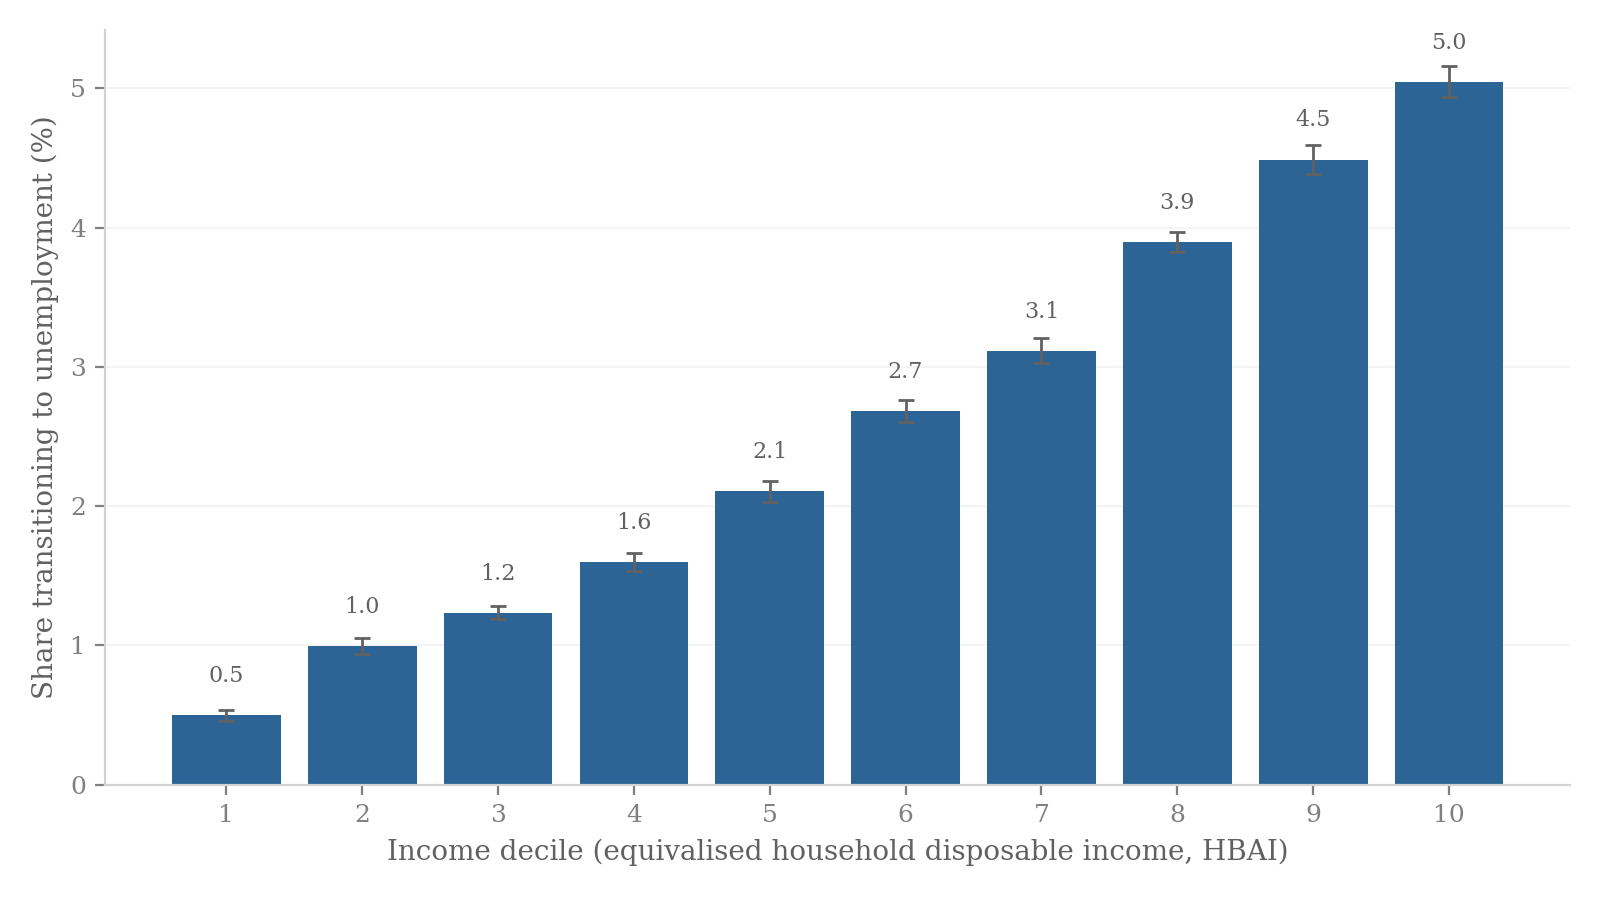
\includegraphics[width=.85\textwidth]{../results/jr16/fig4_1_transition.png}
\caption{Share of the population transitioning from employment to unemployment by equivalised disposable income decile, central scenario. Bars are means over 50 seeded displacement draws; error bars show central 95 per cent intervals across assignment draws. The gradient reflects the exposure-proportional allocation assumption, not observed incidence (see text).}
\label{fig:transition}
\end{figure}

The wage channel, by contrast, is almost distributionally flat. Figure~\ref{fig:wages} shows the percentage change in employment income among workers who remain employed: gains run from 2.50 per cent in the bottom decile to 2.72 per cent in the top, % results/jr16/fig4_2_wage_gain_by_decile.csv
a spread of barely 0.2 percentage points around the 2.6 per cent average uplift. Exposure is sufficiently widespread across the deciles in which people work that the productivity dividend is spread thinly and evenly. Under the central design, most cross-decile variation comes from the displacement margin. That allocation is a property of the scenario design rather than a finding: in the US evidence of \citet{acemoglu2022tasks}, task displacement operates chiefly through relative wage declines, which account for 50--70 per cent of changes in the wage structure. Section~\ref{sec:results-wagemargin} examines this alternative: a wage-margin implementation of the same headline calibration shifts losses from benefit caseloads to earnings, with a comparable fiscal cost but an almost entirely different poverty and inequality profile.

\begin{figure}[htbp]
\centering
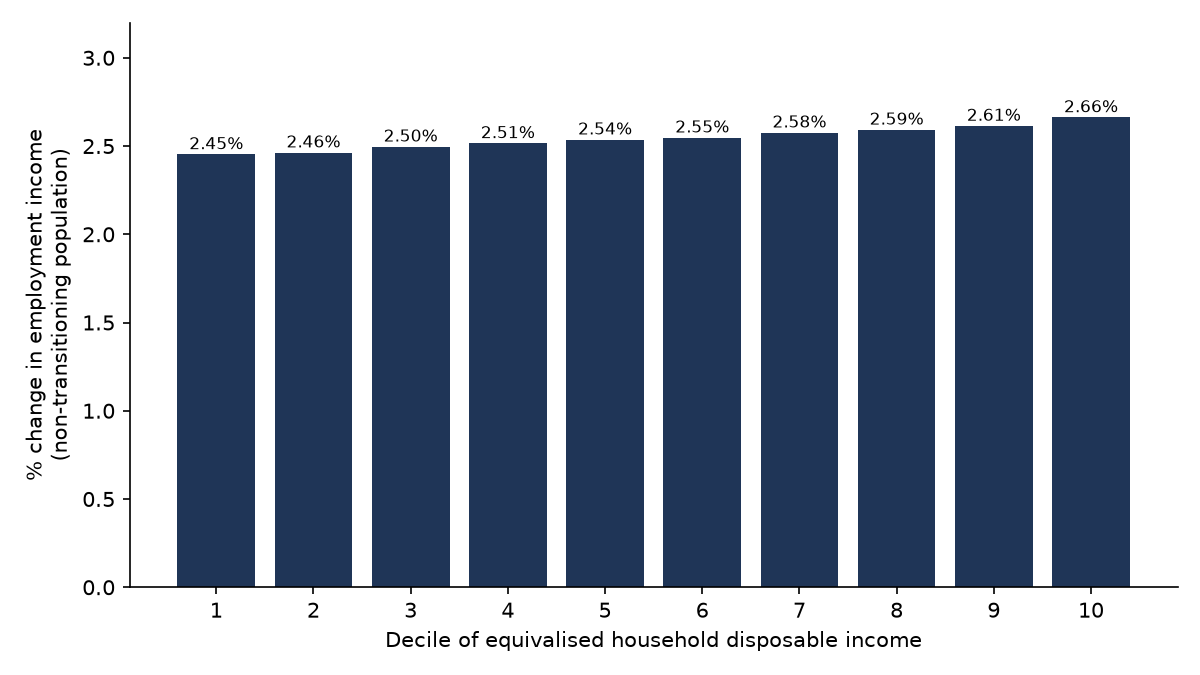
\includegraphics[width=.85\textwidth]{../results/jr16/fig4_2_wages.png}
\caption{Percentage change in employment income among workers remaining in employment, by income decile, central scenario. Means over 50 seeded draws.}
\label{fig:wages}
\end{figure}

The third channel is capital income. The scenario assumes part of the productivity gain is capitalised into returns on existing capital, applying a uniform proportional uplift to interest and dividend income (Section~\ref{sec:shocks}). Although the percentage change is identical across deciles by construction, Figure~\ref{fig:capital} shows the incidence in pounds is heavily concentrated: the top decile holds 35.2 per cent of all capital income (\pounds 8.1 billion of the baseline aggregate in my data), the top two deciles together more than half, and the bottom decile just 2.8 per cent. Under this proportional allocation, most simulated capital-income gains accrue to households already near the top of the distribution.

\begin{figure}[htbp]
\centering
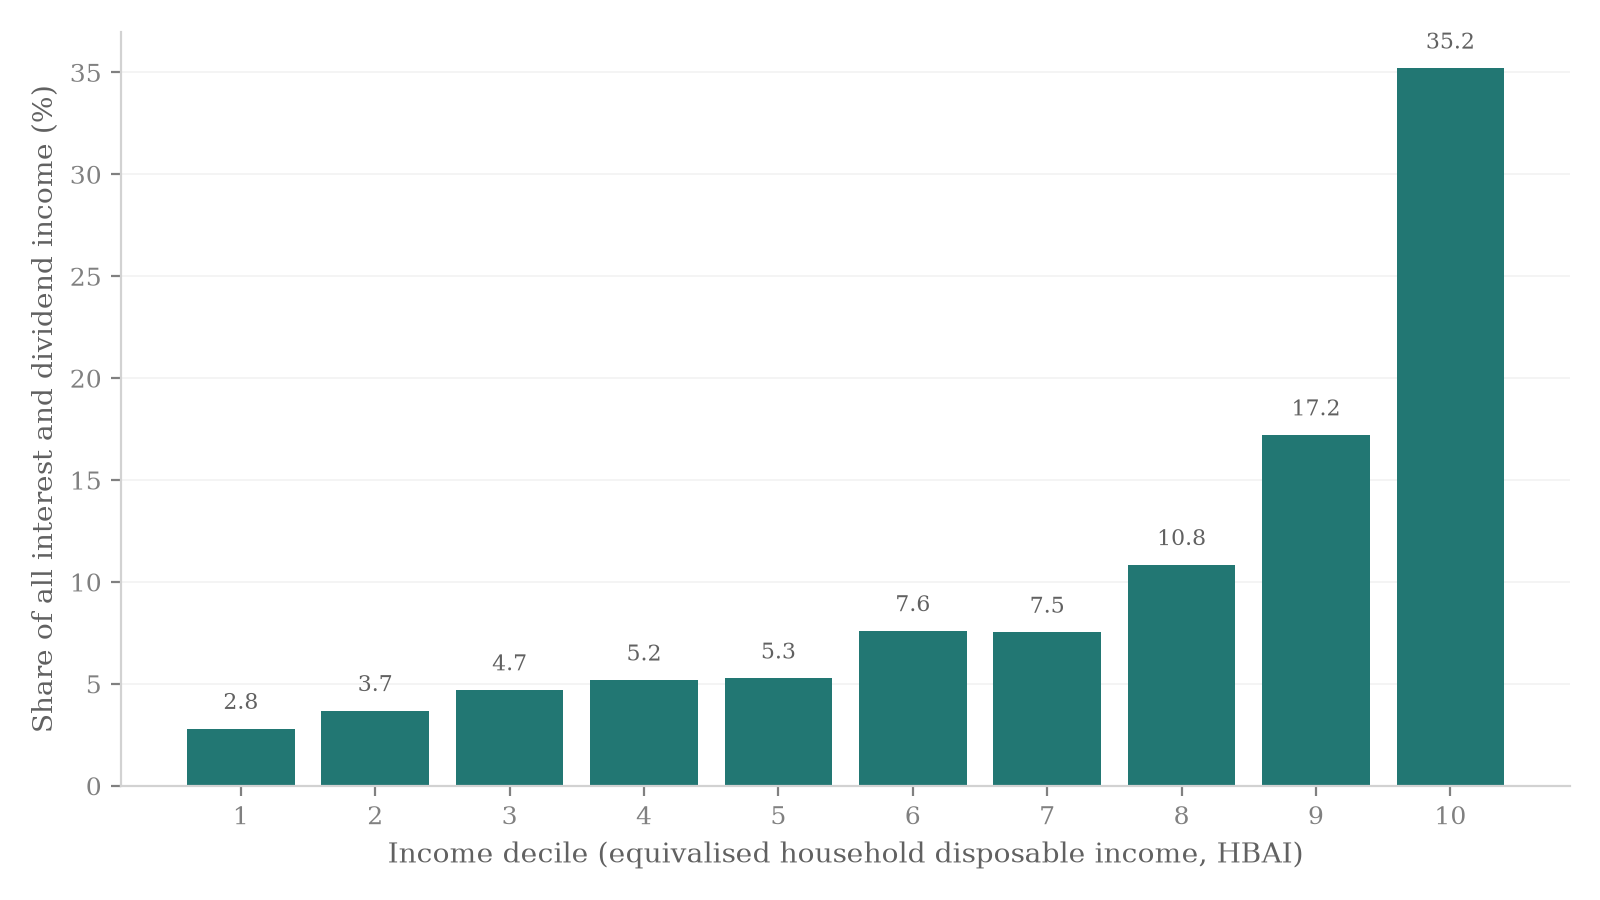
\includegraphics[width=.85\textwidth]{../results/jr16/fig4_3_capital.png}
\caption{Capital income channel by decile: a uniform proportional uplift, but pound gains concentrated where capital income is held.}
\label{fig:capital}
\end{figure}

\subsection{Household mediation of the shock}
\label{sec:results-mediation}

The tax-benefit system converts each market-income loss into a smaller disposable-income loss; Figure~\ref{fig:decomp} decomposes that mediation by decile into market income, benefits, and taxes and contributions, all expressed relative to baseline disposable income. The decomposition is household-level and additive: market income change plus benefit change minus tax change equals the disposable income change up to an explicit residual, which collects perimeter items inside the HBAI concept (council tax and pension deductions) and never exceeds 0.5 per cent of baseline income in any decile.

Market income losses follow the transition gradient: they are near zero in the bottom decile, around 0.8--2.0 per cent of baseline disposable income in deciles 3--5, between 3.3 and 4.1 per cent in deciles 7--9, and reach 6.7 per cent in the top decile. The tax-benefit system then cushions these losses through two distinct mechanisms. Across the middle deciles, automatic benefit entitlements---Universal Credit in particular---rise by up to 0.4 per cent of baseline income as displaced earners qualify for means-tested support. At the top the cushioning operates through the tax system instead: deciles 7--10 see their income tax and National Insurance liabilities fall by 0.4--2.0 per cent of baseline income as high-marginal-rate earnings disappear. The combined offset is substantial. In decile 10, a market income loss of 6.7 per cent of baseline disposable income becomes a disposable income loss of 4.3 per cent---roughly a third of the market shock absorbed---and in decile 5 a 1.8 per cent market loss becomes a 1.1 per cent disposable loss. Averaged over 20 displacement draws, disposable income losses run from 0.75 per cent in the bottom decile to 3.87 per cent in the top; the gradient is upward and stable across draws, though on the current 20-draw means it is not everywhere strictly monotone: decile 3 loses slightly less than decile 2 ($-0.85$ against $-0.93$ per cent) and deciles 9 and 10 are essentially tied ($-3.87$ per cent each), both differences well inside the draw noise. % seed-0 components from results/jr16/fig4_4_decomposition.csv; 20-draw means from results/appendix/decomposition_ci.csv

\begin{figure}[htbp]
\centering
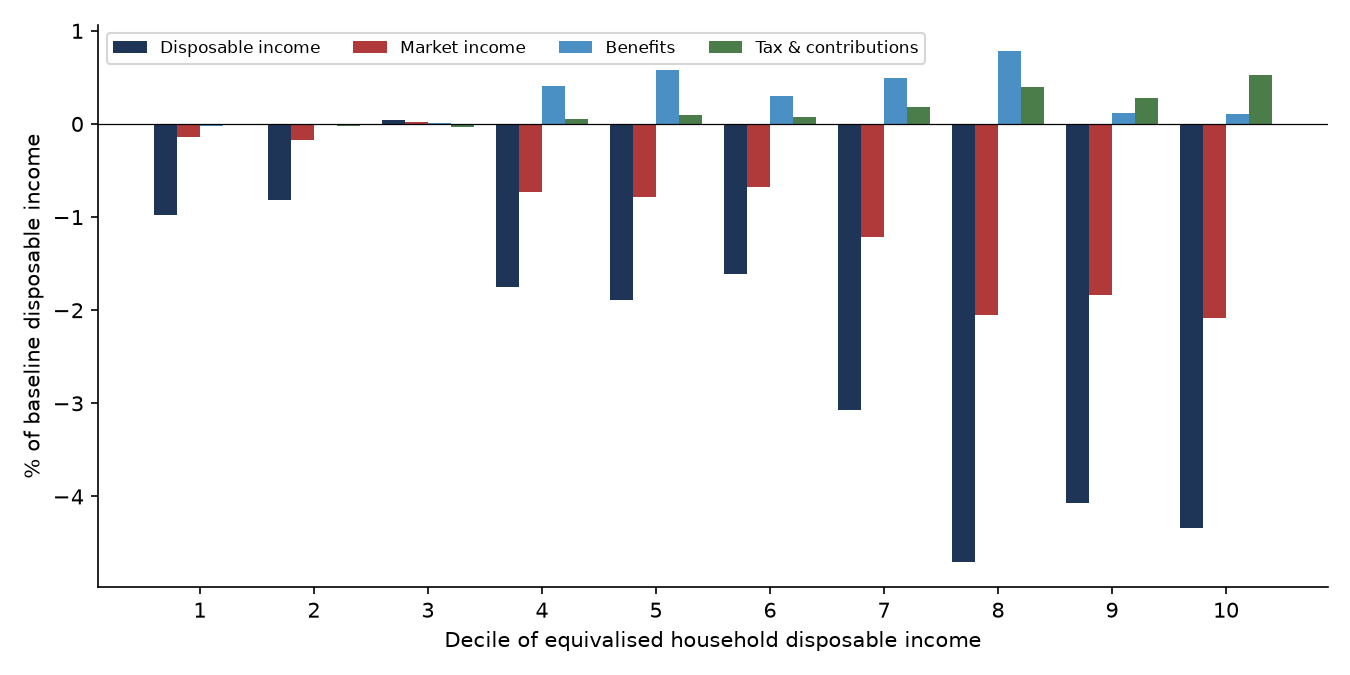
\includegraphics[width=.85\textwidth]{../results/jr16/fig4_4_decomposition.png}
\caption{Additive household-level decomposition of the change in income by decile into market income, benefits, and taxes and contributions, central scenario (single draw, seed 0), as a share of baseline HBAI disposable income. The residual collects perimeter items (council tax, pension deductions) inside the HBAI concept.}
\label{fig:decomp}
\end{figure}

\subsection{Fiscal and distributional aggregates}
\label{sec:results-aggregates}

Table~\ref{tab:presets} summarises the preset scenarios. In the central scenario the annual Exchequer cost is \pounds \genCentralCostBn~billion, driven by lost income tax and National Insurance on displaced higher earners together with higher benefit spending. Poverty rises by \genCentralPovBhcPp~percentage points before housing costs (\genCentralPovAhcPp~points after housing costs) and the Gini coefficient of equivalised disposable income rises by \genCentralGiniChangePp~percentage points from a baseline of \genBaselineGini. The low scenario---a 1 per cent displacement rate with no wage gain, which I treat purely as a sensitivity case rather than an estimate drawn from the literature---costs \pounds \genLowCostBn~billion and moves poverty and the Gini by roughly 0.2--0.3 points each. The high scenario, at 13 per cent displacement, costs \pounds \genHighCostBn~billion a year with poverty up \genHighPovBhcPp~points. PolicyEngine's before-housing-costs poverty line is an \emph{absolute} threshold, so these poverty changes measure absolute impoverishment rather than movement relative to a shock-shifted median. On the relative (60 per cent of contemporaneous median) BHC line the central scenario raises poverty by $+0.71 \pm 0.16$ percentage points over 50 draws --- well under half the absolute-line rise, because the shock lowers the median itself and so drags the relative line down with it. % results/robustness/central_monte_carlo.json relative_poverty_change_bhc_pp

The scenario anchors deserve a note of caution. The central calibration converts the task-exposure and productivity figures of \citet{briggs2023} into a displacement rate and a wage uplift via the conventions described in Section~\ref{sec:scenarios}; it is a calibration convention, not a forecast. The low scenario is likewise not an employment estimate from \citet{acemoglu2025}, whose 0.9--1.1 per cent figure refers to ten-year GDP growth, not job displacement.

\begin{table}[htbp]
\centering
\caption{Summary of preset scenarios (single draw, seed 0)}
\label{tab:presets}
\small
\begin{tabular}{lrrrr}
\toprule
Scenario & Displaced & Exchequer & $\Delta$ Poverty & $\Delta$ Gini \\
 & (million) & (\pounds bn/yr) & (BHC, pp) & (pp) \\
\midrule
Low & 0.24 & 4.3 & +0.33 & +0.21 \\
Central & 1.56 & 18.2 & +1.81 & +1.04 \\
High & 3.04 & 46.9 & +4.05 & +2.07 \\
% source: results/low.json, results/central.json, results/high.json (seed 0)
\bottomrule
\end{tabular}

\vspace{0.4em}
\parbox{0.92\textwidth}{\footnotesize\emph{Note:} Low: 1 per cent displacement, no wage gain (sensitivity case). Central: 7 per cent displacement, 2.6 per cent wage gain. High: 13 per cent displacement, 2.6 per cent wage gain. The capital-return shock (+0.4pp) applies in every preset.}
\end{table}

The central estimates are similar, but not identical, across the 50 assignment draws: the mean Exchequer cost is \pounds \genCentralMcCostMeanBn~billion (assignment-draw standard deviation \pounds \genCentralMcCostSdBn~billion; range \pounds \genCentralMcCostMinBn--\genCentralMcCostMaxBn~billion), with mean poverty and Gini increases of $\genCentralMcPovBhcMeanPp \pm \genCentralMcPovBhcSdPp$ and $\genCentralMcGiniMeanPp \pm \genCentralMcGiniSdPp$ percentage points. In the alternative indices tested, headline estimates change moderately: replacing C-AIOE with the DSIT AIOE mapping leaves the seed-0 Exchequer cost essentially unchanged, while the GPT-exposure measure of \citet{eloundou2023} raises it by about \pounds 2.2 billion (12 per cent); both produce similar upward transition gradients (Appendix~\ref{app:index-sensitivity}). % results/robustness/index_sensitivity_full.json

Two tested assumptions materially change the headline numbers. The first is displacement duration. The central scenario removes a full year of earnings from every displaced worker; under a 50 per cent earnings-retention hybrid---annual earnings are halved while employment status and hours remain those of full-year unemployment, so this approximates rather than models a six-month spell---the Exchequer cost falls from \pounds \genCentralMcCostMeanBn~billion to \pounds \genDurSixMoCostMeanBn~$\pm$~\genDurSixMoCostSdBn~billion and the BHC poverty rise all but vanishes ($+\genDurSixMoPovBhcMeanPp \pm \genDurSixMoPovBhcSdPp$ points), over 20 draws. The collapse is more than proportional---a na\"ive halving of the full-year result would give \pounds 8.9 billion---because workers who keep half a year's earnings remain taxpayers and largely stay clear of means-tested support. Every fiscal and poverty magnitude in this paper therefore scales strongly with the expected out-of-work duration, and the headline figures should be read as a full-year no-reemployment case. The second is benefit take-up. Imposing a 70 per cent Universal Credit take-up probability (drawn identically in baseline and shocked worlds) moves the cost to \pounds \genTakeupCostMeanBn~$\pm$~\genTakeupCostSdBn~billion and the poverty rise to $+\genTakeupPovBhcMeanPp \pm \genTakeupPovBhcSdPp$ points: the headline estimates change little under this single take-up sensitivity. % results/robustness/duration_takeup_sensitivity.json (variant half_earnings_retention; convex-combination comparator 8.86bn)

\subsection{The shock-size grid}
\label{sec:results-grid}

To move beyond the presets I simulate a grid of 66 scenarios, crossing eleven displacement rates (0 to 10 per cent of employees, allocated in proportion to exposure, as in the presets) with six wage uplifts (0 to 5 per cent), each combined with the capital income channel, all under exposure-proportional incidence. Figure~\ref{fig:griddisp} maps the change in average household disposable income. The corners bracket the range: with a 5 per cent wage gain and no job loss, average disposable income rises by 3.0 per cent; with 10 per cent displacement and no wage gain it falls by 5.1 per cent. % results/jr16/grid.csv
The near-zero contour runs close to the grid diagonal---at these calibrations, roughly one percentage point of wage growth offsets one percentage point of displacement in aggregate disposable income terms---so whether AI raises or lowers average living standards is highly sensitive, within this grid, to the balance struck between these two forces, about which the empirical literature remains genuinely uncertain.

\begin{figure}[htbp]
\centering
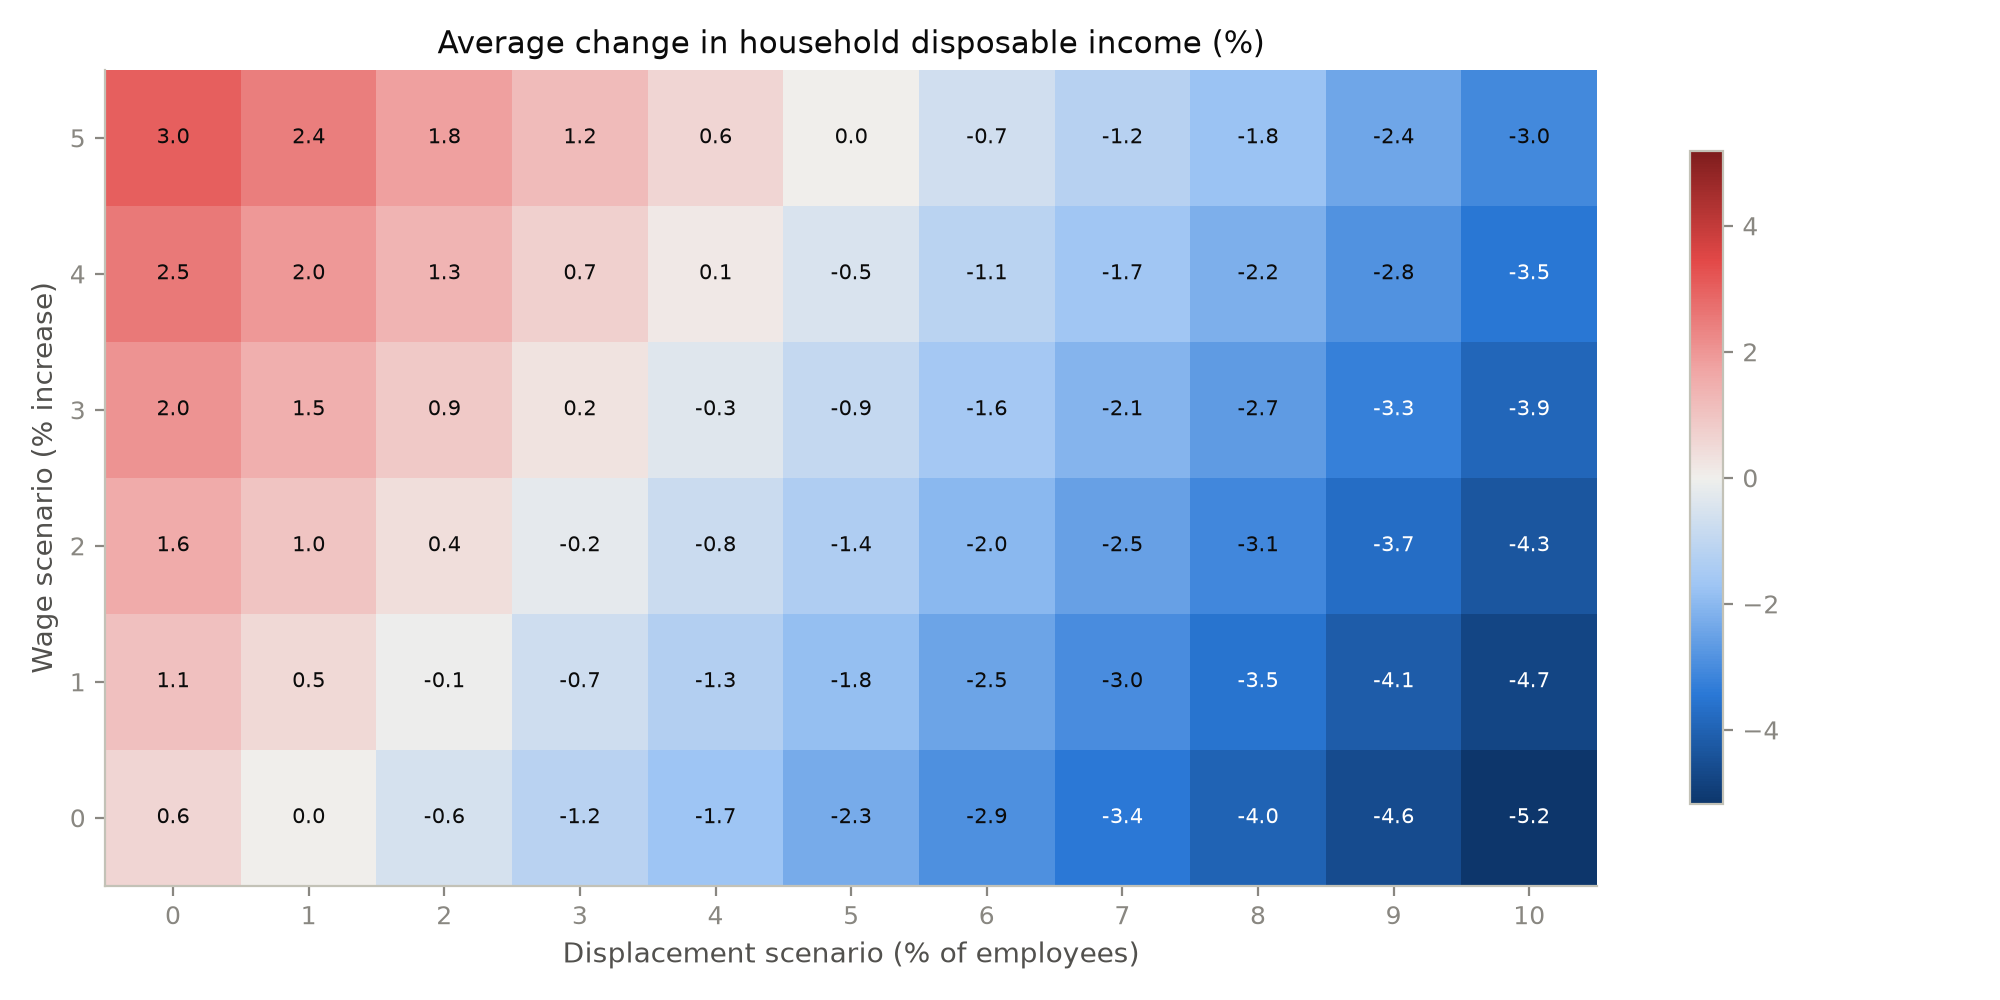
\includegraphics[width=.85\textwidth]{../results/jr16/fig4_5_disposable_grid.png}
\caption{Change in average household disposable income (per cent) across the 66-cell grid of displacement rates and wage uplifts (single draw, seed 0).}
\label{fig:griddisp}
\end{figure}

Figure~\ref{fig:gridrev} shows the corresponding fiscal picture. One measurement issue deserves note: in PolicyEngine's UK aggregates, income tax plus National Insurance minus total benefit expenditure (which includes the state pension) is a negative number, so expressing revenue changes relative to that net position produces uninformative percentages. I therefore express the net revenue change relative to gross income tax and National Insurance receipts as simulated on the household microdata (about \pounds 313 billion); this base is smaller than headline OBR receipts, which include employer contributions and income outside the household survey universe. Two consequences follow. First, the grid's revenue measure is income tax plus National Insurance minus cash benefit expenditure, a narrower concept than the full government-balance measure behind the \pounds \genCentralCostBn~billion headline cost of Section~\ref{sec:results-aggregates}, which also includes indirect taxes and other levies; the grid's cash-tax cost of the central 7 per cent/2.6 per cent scenario is roughly \pounds 11 billion (interpolated between the 2 and 3 per cent wage columns), and the two figures should not be read off the same surface. Second, on that narrower basis the grid spans a gain of \pounds 22.3 billion, or 7.2 per cent of receipts (5 per cent wage growth, no displacement), to a loss of \pounds 29.4 billion, or 9.4 per cent of receipts, in the worst cell (10 per cent displacement, no wage growth). At the central displacement rate, 7 per cent with no wage offset costs \pounds 21.2 billion (6.8 per cent of receipts), which a 3 per cent wage uplift more than halves to \pounds 9.8 billion. % results/jr16/grid.csv
As with disposable income, the break-even locus lies close to the diagonal.

\begin{figure}[htbp]
\centering
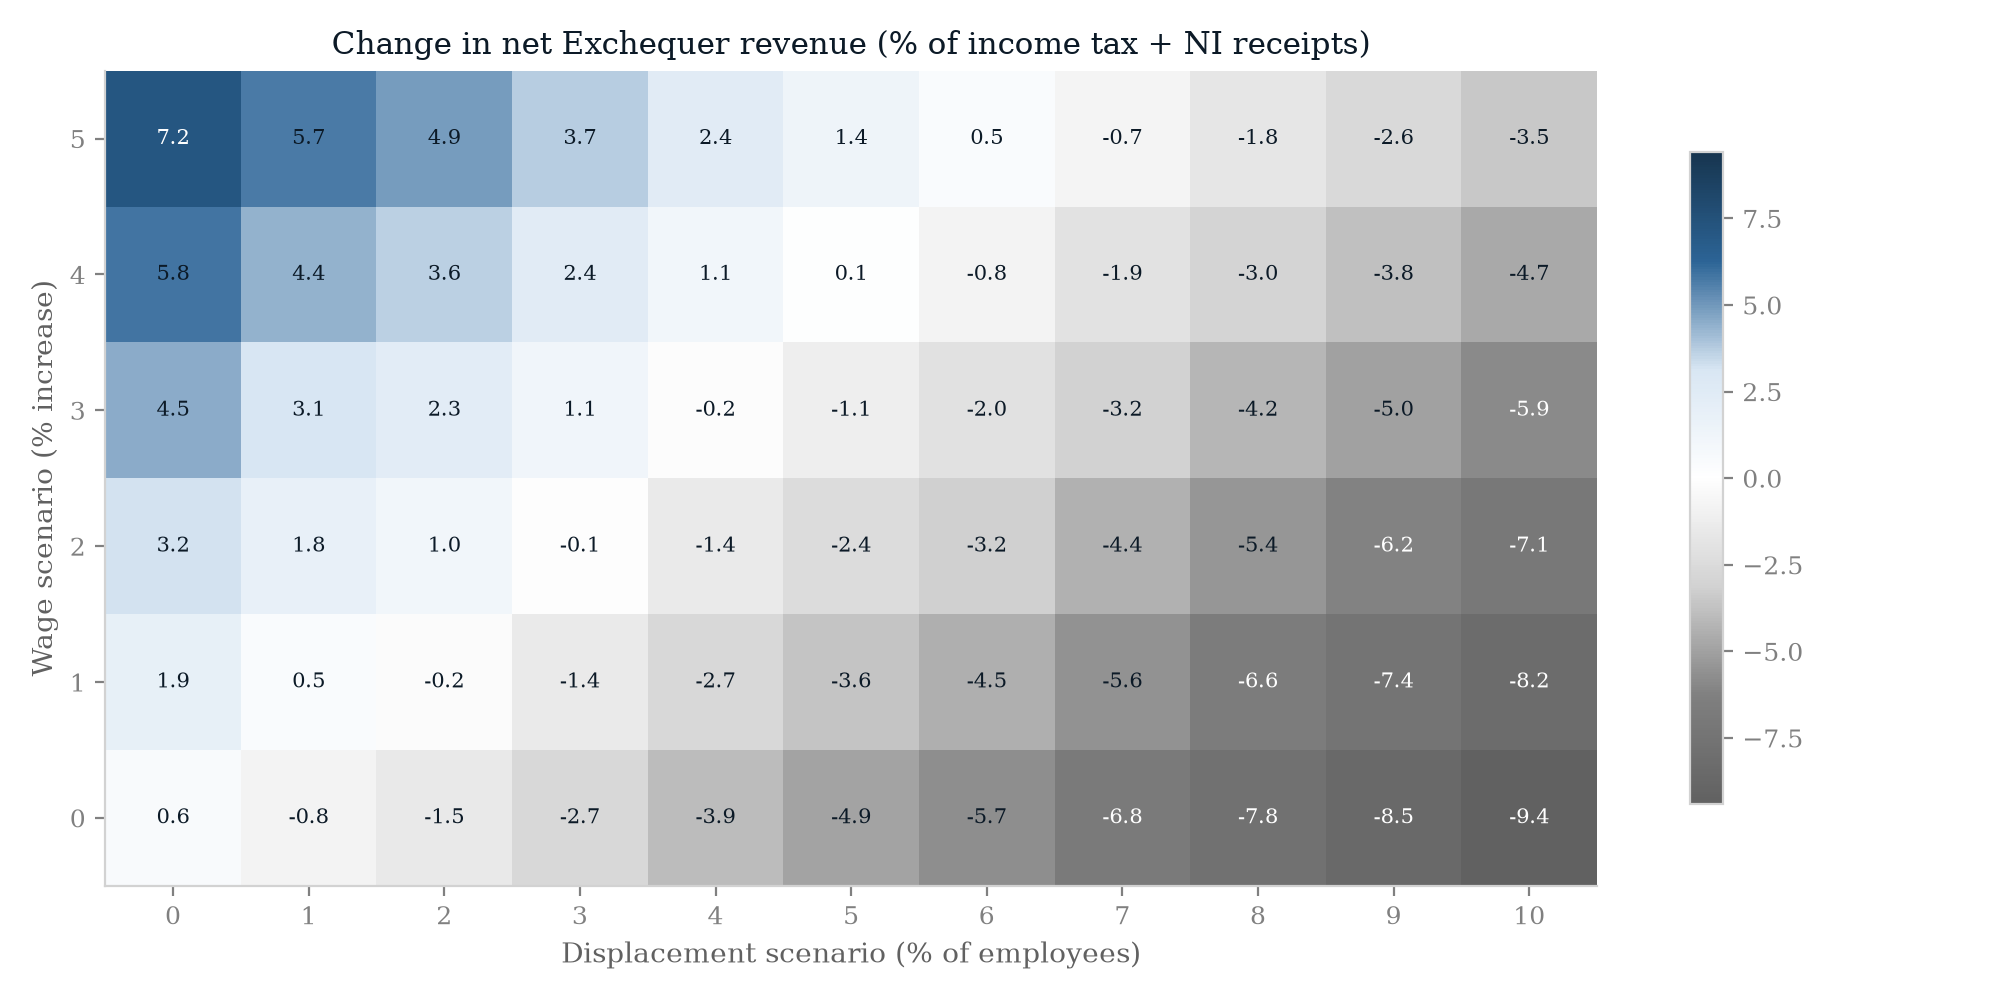
\includegraphics[width=.85\textwidth]{../results/jr16/fig4_6_exchequer_grid.png}
\caption{Net Exchequer revenue change as a percentage of gross income tax and National Insurance receipts, across the 66-cell scenario grid.}
\label{fig:gridrev}
\end{figure}

Figure~\ref{fig:gridgini} maps the change in the Gini coefficient across the same grid, and produces a consistent result within this grid: the Gini rises in all 66 cells, from +\genGridGiniMinPp{} percentage points in the capital-only cell (no displacement, no wage gain) to +\genGridGiniMaxPp{} points at the far corner. No combination of parameters within the grid reduces measured inequality. The simulated pattern is consistent with widening gaps at both ends of the distribution rather than a simple top-income gain, and it coexists with an incidence that is itself progressive: displacement strikes hardest at the top of the earnings ladder and pushes affected households down the distribution, while the wage uplift lifts the surviving employed---disproportionately in the upper-middle and top deciles---further away from workless and low-income households, and the capital channel reinforces the very top. Within the model, losses and gains are allocated in ways that widen gaps between households, and inequality rises even though the market shock lands mainly on higher earners.

\begin{figure}[htbp]
\centering
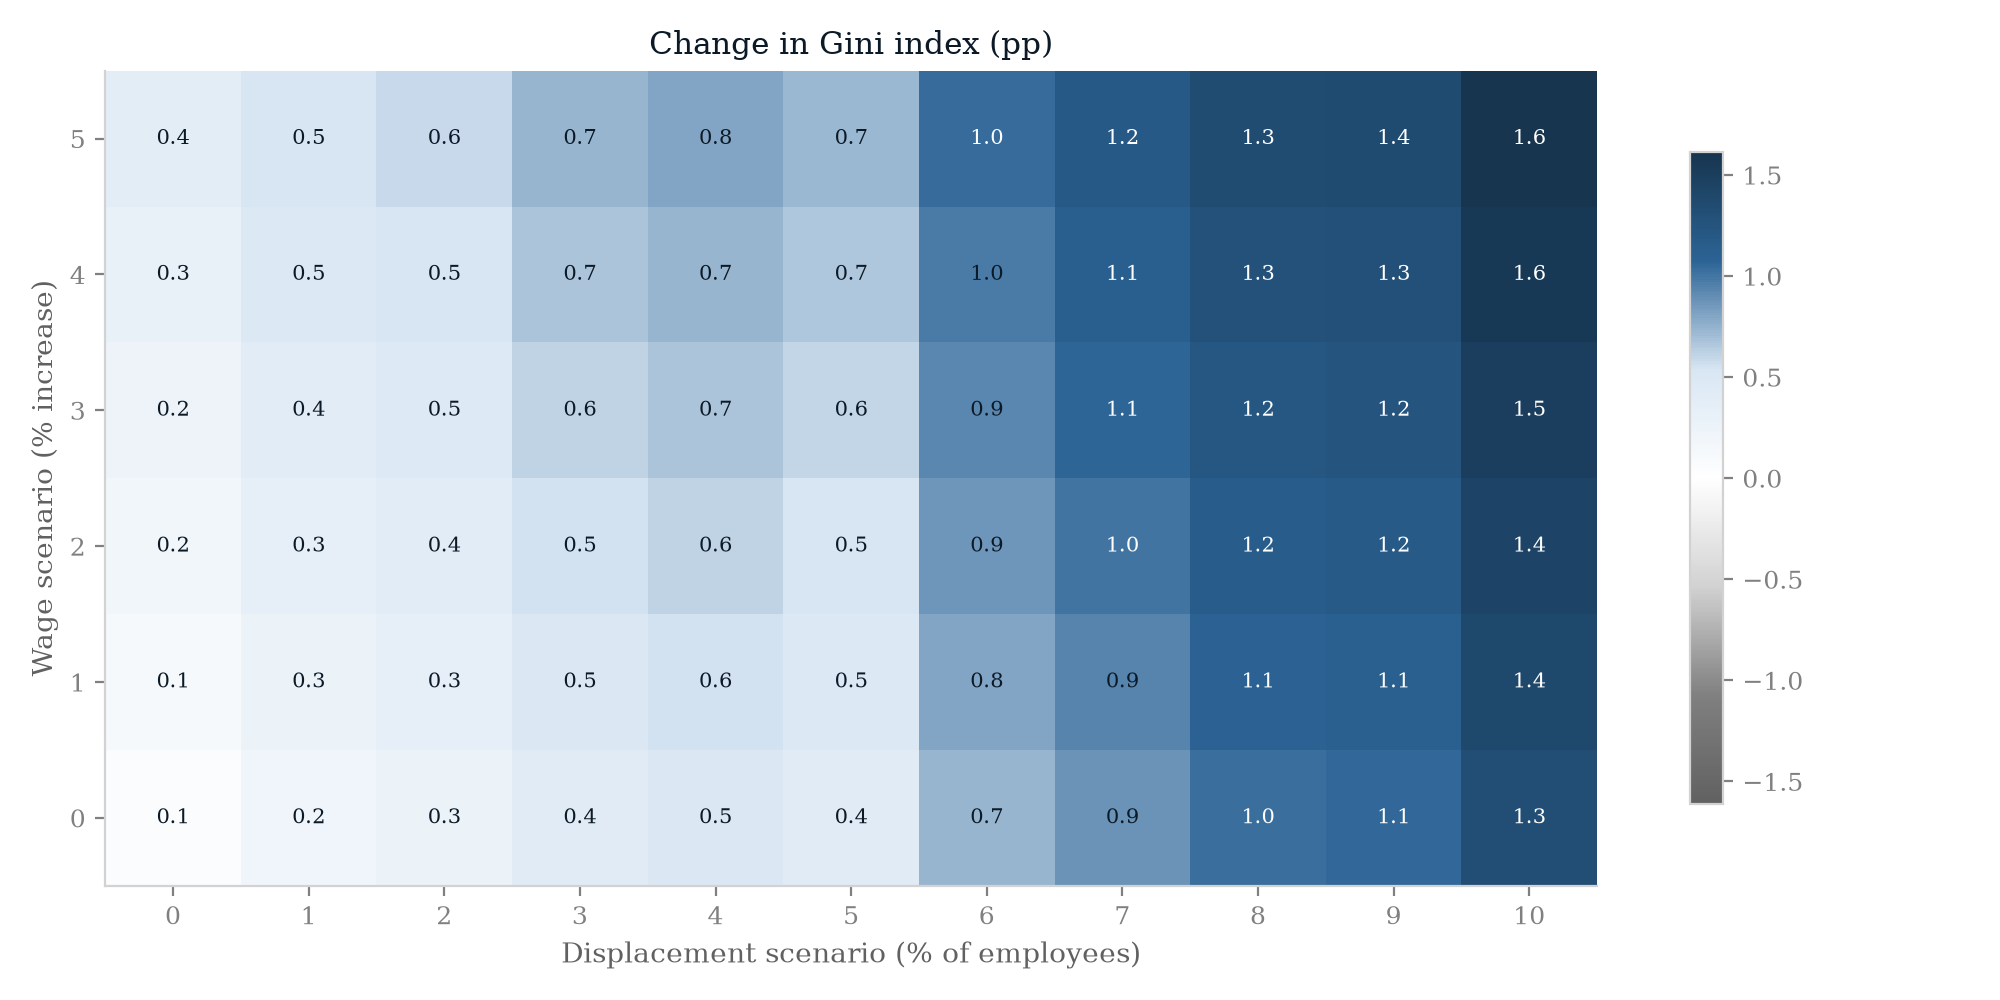
\includegraphics[width=.85\textwidth]{../results/jr16/fig4_7_gini_grid.png}
\caption{Change in the Gini coefficient of equivalised HBAI disposable income (percentage points) across the 66-cell scenario grid. The Gini rises in every cell.}
\label{fig:gridgini}
\end{figure}

\subsection{The incidence axis: who bears the shock}
\label{sec:results-incidence}

Everything so far conditions on exposure-proportional incidence. But allocation is at least as uncertain as shock size, so I reallocate the same central calibration across five families. Four are stylised: exposure-proportional, junior-concentrated, expertise-compression (implemented as a high-earner displacement tilt, not the \citet{hosseinilichtinger2026barriers} wage mechanism; Section~\ref{sec:incidence}) and uniform. The fifth is a Klein-anchored top-loaded stress test: exposure-proportional draws multiplied by an author-imposed junior tilt (1.29) and wage-tier tilt (9.6 above, 0.6 below median person earnings). Table~\ref{tab:incidence} gives means and assignment-draw standard deviations over 50 paired seeds.

\begin{table}[htbp]
\centering
\caption{Central shock under five incidence calibrations}
\label{tab:incidence}
\small
\setlength{\tabcolsep}{5pt}
\renewcommand{\arraystretch}{1.12}
\begin{tabular}{lrrrr}
\toprule
Incidence family & Displaced & Exchequer cost & $\Delta$ Poverty & $\Delta$ Gini \\
 & (million) & (\pounds bn/yr) & BHC (pp) & (pp) \\
\midrule
Exposure-proportional & 1.56 & 17.7 $\pm$ 1.2 & +1.87 $\pm$ 0.15 & +1.11 $\pm$ 0.09 \\
Junior-concentrated & 1.55 & 17.9 $\pm$ 1.6 & +1.85 $\pm$ 0.14 & +1.08 $\pm$ 0.08 \\
Expertise-compression & 1.67 & 20.6 $\pm$ 1.8 & +1.96 $\pm$ 0.15 & +1.04 $\pm$ 0.09 \\
Uniform & 1.55 & 13.9 $\pm$ 1.7 & +1.87 $\pm$ 0.17 & +1.16 $\pm$ 0.10 \\
Klein-anchored stress test & 1.62 & 32.8 $\pm$ 2.2 & +2.24 $\pm$ 0.14 & +0.97 $\pm$ 0.12 \\
% source: results/robustness/incidence_monte_carlo.json (means/sd); displaced from results/incidence/summary_five.csv (seed 0)
\bottomrule
\end{tabular}

\vspace{0.4em}
\parbox{0.92\textwidth}{\footnotesize\emph{Note:} Means $\pm$ assignment-draw standard deviations over 50 paired seeds. Assignment quantiles and Monte Carlo standard errors are reported separately in the machine-readable summary; they describe allocation noise, not population uncertainty. The Klein-anchored family combines exposure with author-imposed junior (1.29) and wage-tier (9.6 above / 0.6 below median person earnings) multipliers. The wage-tier values use press-release maximum-exposure scalings rather than the paper's per-standard-deviation estimates; this is a stress test, not an estimated displacement schedule. AHC poverty is evaluated on the same 50 draws as BHC poverty and the Gini.}
\end{table}

\begin{figure}[htbp]
\centering
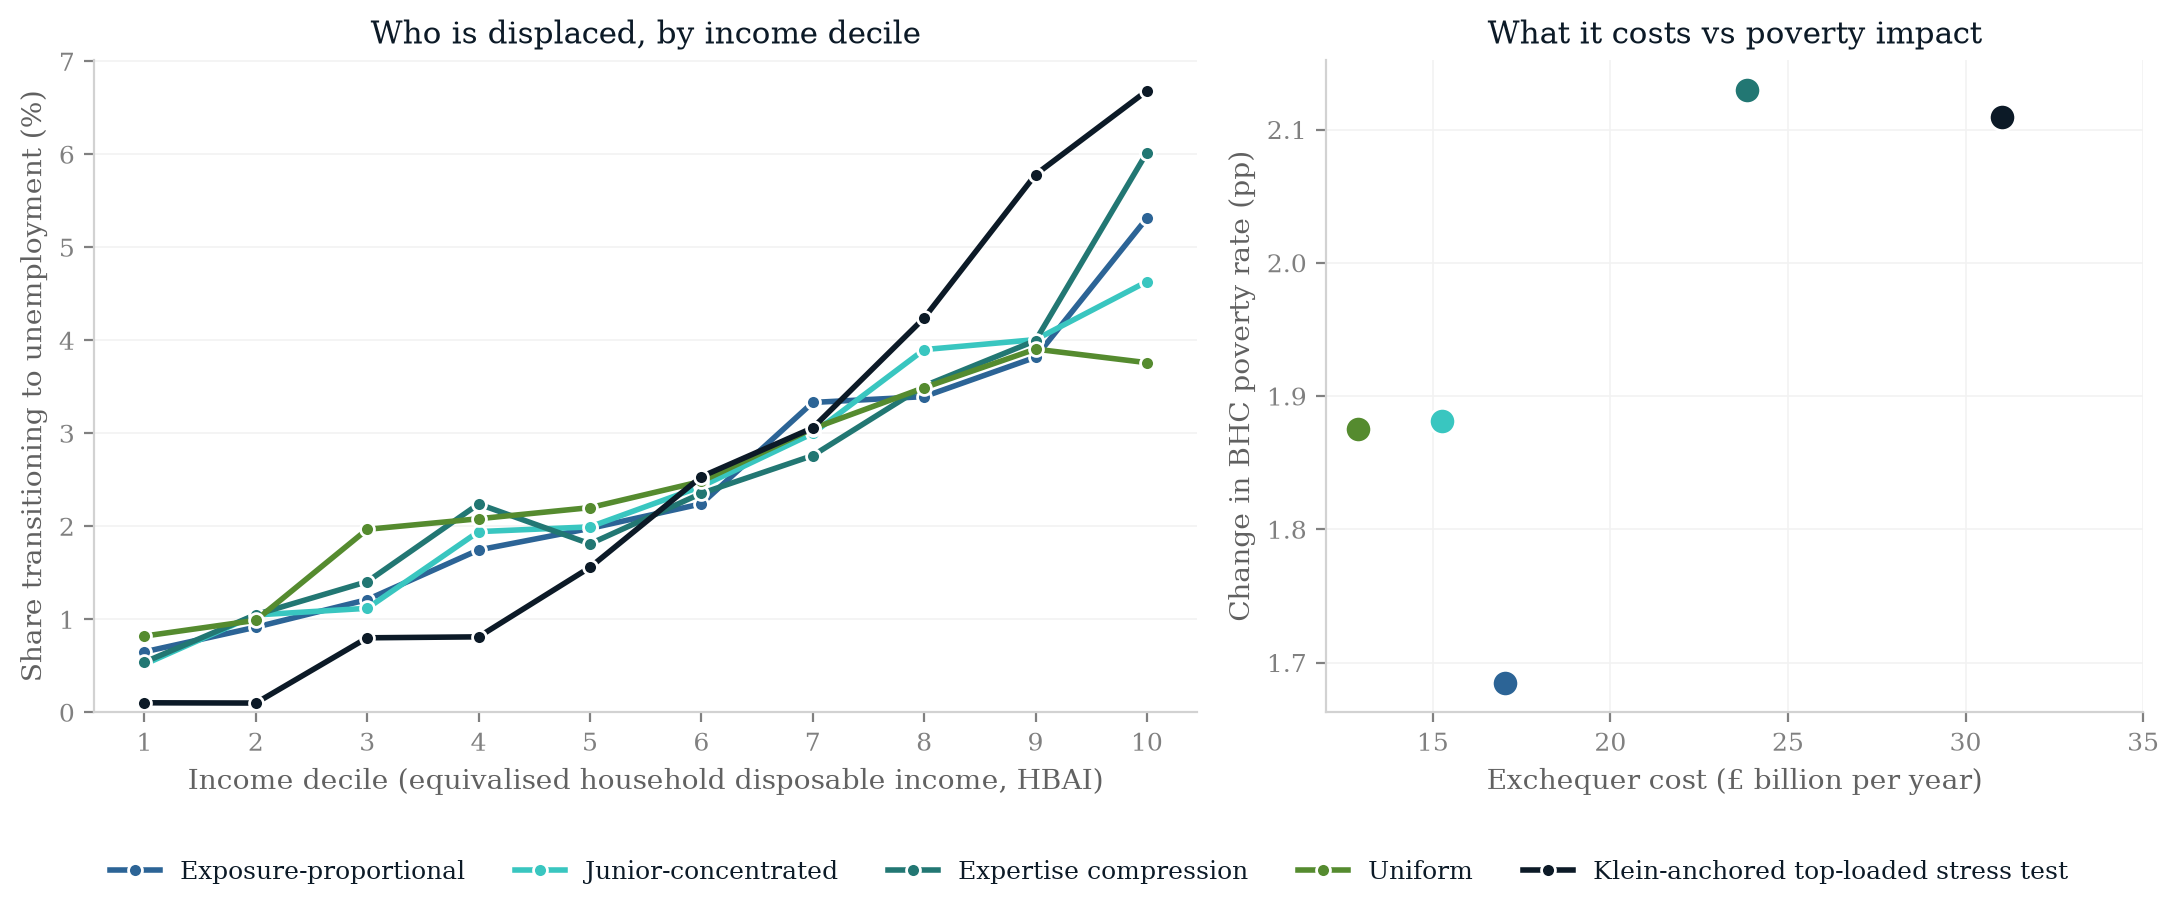
\includegraphics[width=.95\textwidth]{../results/incidence/incidence_families.png}
\caption{Decile incidence of the same aggregate central shock under five incidence families: share of each decile transitioning to unemployment, and change in equivalised HBAI disposable income by decile. The figure shows a single illustrative draw (seed 0), whereas the aggregates in Table~\ref{tab:incidence} are means over 50 Monte Carlo draws.}
\label{fig:incidence}
\end{figure}

Within these calibrations, who bears the shock materially changes its simulated cost. The mean Exchequer cost ranges from \pounds \genIncUniformCostMeanBn~billion under uniform incidence to \pounds \genIncKleinCostMeanBn~billion under the Klein-anchored stress test, generated by reallocating which workers lose their jobs. The larger fiscal effects under top-loaded incidence are consistent with the larger tax liabilities of the displaced high earners. These are paired-seed scenario comparisons, not population confidence statements.

% Paired 95% intervals recomputed from results/robustness/incidence_draws_five.csv (clean-room rebuild vintage; paired normal interval on draw-level differences, 50 shared seeds).
Across the four stylised families, the mean BHC poverty rise lies between \genIncFamilyPovBhcMeanMinPp{} and \genIncCompressionPovBhcMeanPp{} percentage points, while mean Exchequer costs span nearly \pounds 7 billion. Because the families share assignment seeds, draw-level \emph{differences} support paired inference: the expertise-compression poverty effect exceeds the exposure-proportional one by $+0.09$ points (paired 95 per cent interval $[+0.03, +0.15]$). The uniform--exposure poverty difference is indistinguishable from zero ($-0.00$ points, $[-0.06, +0.06]$); all families share the central wage and capital axis, so the comparison isolates displacement allocation. Uniform incidence retains a reliably smaller fiscal effect than exposure-proportional incidence ($-\pounds 3.84$ billion, $[-4.46, -3.21]$) alongside a reliably larger Gini effect (below). The junior-concentrated and exposure-proportional fiscal costs remain indistinguishable under the same paired comparison ($+\pounds 0.19$ billion, $[-\pounds 0.30, +\pounds 0.67]$). These paired intervals describe assignment-draw noise only, not population sampling uncertainty.

The author-imposed top-loaded calibrations combine relatively large fiscal and poverty effects. Expertise compression costs \pounds \genIncCompressionCostMeanBn~billion and raises BHC poverty by +\genIncCompressionPovBhcMeanPp{} points. The Klein-anchored stress test has means of \pounds 32.8 billion and +2.24 points; its AHC effect is evaluated over the same 50 assignment draws. Its wage-tier multiplier produces the most top-tilted seed-0 gradient, from 0.01 per cent transitioning in the bottom decile to 7.25 per cent in the top. These magnitudes are conditional on the stress-test mapping and are not estimates transported from Klein Teeselink.

The Gini rises in all five simulated families---50-draw means of +\genIncFamilyGiniMeanMinPp{} to +\genIncFamilyGiniMeanMaxPp{} percentage points---just as it rises in all 66 grid cells (in the appendix's capital-off variant of the grid the null cell with no shock at all is exactly zero, as it must be). Paired inference again separates some families: the uniform Gini effect exceeds the exposure-proportional one by $+0.04$ points (paired 95 per cent interval $[+0.01, +0.08]$), and the Klein-anchored Gini effect is reliably \emph{smaller} than the expertise-compression one ($-0.07$ points, $[-0.12, -0.03]$), consistent with its more top-concentrated losses compressing the upper tail. % paired intervals from results/robustness/incidence_draws_five.csv (50 shared seeds)
The directional result is explicitly conditional on these displacement calibrations.

\subsection{The adjustment margin: wage cuts versus displacement}
\label{sec:results-wagemargin}

The incidence families reallocate displacement across workers; the wage-margin family instead moves the same shock to the wage margin. Every employee keeps their job, and earnings are removed through author-imposed occupation-level cuts proportional to C-AIOE or PSS, calibrated so that the aggregate employee-earnings loss equals the realised gross earnings loss of the paired central displacement draw---7.77 per cent of the baseline wage bill at seed 0 (recorded target share 0.07774), larger than the 7 per cent head-count rate because group job-loss rates correlate with group pay; the equality is asserted in code. The PSS rows are a PSS-ranked wage-cut stress test, not the \citet{hosseinilichtinger2026barriers} labour-supply mechanism. Table~\ref{tab:wagemargin} compares these clearly labelled calibrations on the seed-0 basis. % results/wage_margin_central.json gross_cut_share_target = 0.07773605...

\begin{table}[htbp]
\centering
\caption{The headline calibration on two adjustment margins (central calibration; displacement row single draw, seed 0; wage-margin rows deterministic)}
\label{tab:wagemargin}
\small
\begin{tabular}{lrrr}
\toprule
Scenario & Exchequer cost & $\Delta$ Poverty & $\Delta$ Gini \\
 & (\pounds bn/yr) & BHC (pp) & (pp) \\
\midrule
Central displacement & 18.2 & +1.81 & +1.04 \\
Wage margin (C-AIOE gradient) & 26.6 & +0.10 & $-$0.44 \\
Wage margin (PSS gradient) & 26.4 & +0.17 & $-$0.35 \\
% source: results/central.json, results/wage_margin_central.json, results/wage_margin_pss.json
\bottomrule
\end{tabular}

\vspace{0.4em}
\parbox{0.92\textwidth}{\footnotesize\emph{Note:} The wage-margin rows remove the same aggregate gross earnings as the paired seed-0 central displacement draw (7.77 per cent of the baseline employee wage bill); the displacement row removes the earnings of a weighted 7 per cent of employees. All rows apply the 2.6 per cent wage uplift and the capital shock. The wage-margin scenarios displace no one: cuts are occupation-level percentages proportional to the stated gradient, calibrated to the stated baseline-wage-bill share. After-housing-costs poverty changes are +1.85, +0.27 and +0.35 points respectively.}
\end{table}

Three contrasts stand out. First, under the simulated wage schedules the fiscal cost rises from \pounds \genCentralCostBn~billion to \pounds \genWageMarginCentralCostBn~billion (\pounds \genWageMarginPssCostBn~billion under the PSS gradient). Wage cuts shave earnings at marginal tax and National Insurance rates, whereas displacement removes whole earnings blocks and is partly offset by means-tested benefits. This comparison is conditional on these calibrations and does not establish a general lower bound.

Second, the poverty effect all but disappears in the simulated wage-cut cases: the +1.81-point BHC poverty rise becomes +0.10 points under the C-AIOE gradient and +0.17 under PSS. Spreading the calibrated loss across employees pushes fewer households across the frozen absolute line than concentrating losses on displaced workers; this does not establish a bound for other wage schedules.

Third, the sign of the inequality effect flips under both author-chosen wage gradients: the Gini falls by 0.44 and 0.35 points, whereas it rises in the simulated displacement cells. Percentage cuts scale with gradients concentrated in well-paid occupations, compressing earnings from above. The comparison shows that poverty and inequality conclusions depend on both the adjustment margin and its imposed schedule; it does not establish a universal fiscal or distributional result.

Table~\ref{tab:mixedwage} makes the like-for-like comparison. In every row gross earnings loss before the common uplift is 7.77 per cent of the baseline wage bill, exactly the loss realised in the seed-0 central/exposure draw to which the exercise is paired. Moving that fixed loss from wage cuts to displacement reduces the Exchequer cost from \pounds 26.6 billion to \pounds 18.2 billion, while raising BHC poverty from 0.10 to 1.81 points and the Gini effect from $-0.44$ to $+1.04$ points. The half-index case costs \pounds 22.7 billion, raises poverty by 1.02 points and raises the Gini by 0.29 points. Net employee-income losses after the uplift rise slightly, from 5.11 to 5.32 per cent, because fewer survivors receive the uplift as displacement rises; the pre-uplift loss being compared is invariant. % results/robustness/mixed_adjustment.csv
Conditional on this author-designed allocation rule, the monotone poverty and inequality patterns track the shifting adjustment margin; they are not structural causal estimates.

\begin{table}[htbp]
\centering
\caption{Adjustment-margin and survivor-wage sensitivities (seed 0, 2026)}
\label{tab:mixedwage}
\small
\begin{tabular}{lrrrr}
\toprule
Scenario & Displaced & Exchequer cost & $\Delta$ Poverty & $\Delta$ Gini \\
 & (million) & (\pounds bn/yr) & BHC (pp) & (pp) \\
\midrule
\multicolumn{5}{l}{\emph{Fixed gross earnings loss (7.77 per cent); $\lambda$ scales displacement}} \\
$\lambda=0$ & 0.00 & 26.6 & +0.10 & $-$0.44 \\
$\lambda=.25$ & 0.42 & 24.5 & +0.61 & $-$0.03 \\
$\lambda=.50$ & 0.77 & 22.7 & +1.02 & +0.29 \\
$\lambda=.75$ & 1.15 & 20.6 & +1.39 & +0.62 \\
$\lambda=1$ & 1.56 & 18.2 & +1.81 & +1.04 \\
\midrule
\multicolumn{5}{l}{\emph{Central 7 per cent displacement with alternative survivor-wage effects}} \\
$-5.0\%$ & 1.56 & 57.3 & +2.65 & +0.59 \\
$-2.6\%$ & 1.56 & 45.0 & +2.21 & +0.73 \\
$0.0\%$ & 1.56 & 31.6 & +2.01 & +0.88 \\
$+2.6\%$ & 1.56 & 18.2 & +1.81 & +1.04 \\
$+5.0\%$ & 1.56 & 5.8 & +1.68 & +1.19 \\
% source: results/robustness/mixed_adjustment.csv, results/robustness/survivor_wage_grid.csv
\bottomrule
\end{tabular}

\vspace{0.4em}
\parbox{0.92\textwidth}{\footnotesize\emph{Note:} In the mixed panel, $\lambda$ thins the central 7 per cent employee-displacement draw and C-AIOE-graded survivor cuts fill the gap to that same seed-0 draw's gross pre-uplift earnings loss (7.77 per cent of the wage bill). Gross loss is identical in every row; the 2.6 per cent complementarity-graded uplift and capital shock then apply. The pure wage-cut endpoint therefore matches the C-AIOE wage-margin row's gross-loss calibration. The second panel holds displaced workers and the capital shock fixed and changes only the employment-weighted survivor-wage parameter. These are author-designed reduced-form comparative statics, not estimates of equilibrium wage responses.}
\end{table}

Allowing survivor wages to fall is more consequential for the level of the fiscal estimate. With the same 1.56 million displaced workers, removing the productivity pass-through raises the Exchequer cost from \pounds 18.2 billion to \pounds 31.6 billion; an average 2.6 per cent wage decline raises it to \pounds 45.0 billion, and a 5 per cent decline to \pounds 57.3 billion. Poverty also rises, but less dramatically, from 1.81 points under the central uplift to 2.65 points under a 5 per cent wage decline, because the additional loss is spread across survivors rather than concentrated as total earnings loss. The assumed positive wage pass-through is a large fiscal offset in this grid. The Gini remains positive in every central-displacement wage cell, including the adverse-wage cases; more positive survivor gains are associated with a larger Gini response, consistent with a wider gap between displaced workers and those who keep their jobs.

\subsection{The age and gender dimensions}
\label{sec:results-agegender}

The incidence axis has a within-family age structure worth drawing out. Under exposure-proportional incidence, workers aged 16--24 account for only 5.3 per cent of the displaced in the central scenario, because young people in the UK are concentrated in low-exposure service occupations; the burden falls on prime-age workers (27.1 per cent of the displaced are aged 35--44). The junior-concentrated family of Table~\ref{tab:incidence} reweights displacement probabilities towards junior workers while holding the aggregate displacement rate at 7 per cent; because juniors are concentrated in occupation groups whose fixed quotas the tilt does not change, the realised seed-0 age composition barely moves (a 16--24 share of 4.8 per cent and a 55--64 share of 18.3 against 18.1 per cent), and the aggregate differences are small relative to variation across the 50 assignment draws for cost (\pounds 17.9 $\pm$ 1.6 under the junior tilt against \pounds 17.7 $\pm$ 1.2 billion under exposure-proportional incidence), poverty and the Gini alike. The exercise shows that the junior tilt is an additional scenario assumption rather than a consequence of occupational exposure alone---and that, within fixed occupation quotas, it does little to redirect the shock towards the young. Even under the junior tilt, prime-age workers remain the largest displaced group. % age shares: results/central.json, results/central_youth_tilted.json (seed 0)

If AI adoption in practice falls hardest on juniors through recruitment rather than dismissal---as the seniority-biased hiring evidence of \citet{hosseini2026} and the early-career employment declines in AI-exposed occupations documented by \citet{brynjolfsson2025} suggest---the fiscal consequences could differ materially from the broad-based scenarios above, because junior workers contribute little income tax and National Insurance. That channel, however, operates through hiring flows that stock-based simulation frameworks such as mine do not capture by construction.

Exposure also carries a gender gradient. Employed women in the FRS have a mean C-AIOE of 0.33 against 0.18 for employed men, reflecting women's concentration in administrative, professional and associate-professional work. In the central scenario this translates into a displacement rate of 7.5 per cent for employed women against 6.5 per cent for men (means over 20 draws): women hold 51.8 per cent of employment but account for 55.4 per cent of the displaced. Household-level income changes are nevertheless similar by sex ($-2.9$ per cent for both women and men). % results/appendix/gender_incidence.json
A natural reading is that income pooling within couples mutes the individual asymmetry at the household level, though I have not decomposed the result and offer this as a hypothesis rather than a finding. The individual-level asymmetry itself echoes the international evidence that female employment is substantially more exposed to generative AI than male employment \citep{ilo2025}.

\subsection{Benefit caseloads}
\label{sec:results-caseloads}

The fiscal aggregates above can also be read on the delivery side, as caseloads. In the central scenario the shock draws 370,000 benefit units into Universal Credit while 59,000 exit, a net caseload increase of \genCaseloadNetNewUcBenunitsK,000 benefit units, and annual UC spending rises by \pounds \genCaseloadUcSpendChangeBn~billion from a baseline of \pounds 41.4 billion, of which \pounds 0.4 billion is the housing element within paid awards. Against DWP's roughly \pounds 334 billion of welfare spending in 2025--26 (a context figure, not a model output), the central increment is about 1 per cent; the high scenario roughly doubles it (674,000 net new benefit units, +\pounds 6.3 billion), while the low scenario adds only 30,000 benefit units and \pounds 0.3 billion. Caseload responses vary with incidence in the expected direction: the junior-concentrated family, whose displaced workers more often live in households with other earners, adds fewer benefit units (251,000 net) at lower cost (+\pounds 2.4 billion). Two accounting notes apply: only the benefit-unit figures are net of exits---the corresponding household and person counts (353,000 and \genCaseloadNewUcPersonsK,000 in the central scenario) are gross new entrants---and the housing element is measured within paid awards, slightly overstating housing-specific cash. % results/caseloads/summary.csv

\section{Policy responses}
\label{sec:policy}

If the shock modelled above is structural rather than cyclical---a permanent reallocation of labour demand rather than a downturn that unwinds---then the question facing the state is not whether the existing tax-benefit system cushions the blow (Section~\ref{sec:results} shows that it does, absorbing roughly half of the market-income loss) but whether it cushions it well, and at what fiscal cost the residual hardship could be bought down. This section evaluates three stylised policy responses inside the shocked world. Each reform is simulated on top of the central scenario (7 per cent displacement, seed 0, 2026), so the estimand throughout is the difference between the shocked-plus-reform and shocked simulations: what the reform adds, given that the shock has happened. I make no claim about the merits of these instruments in the absence of the shock, and the reforms apply for 2026 only---they are circuit breakers, not permanent settlements.

\subsection{Three stylised reforms}
\label{sec:policy-reforms}

The first reform (R1) is a wage-insurance scheme in the spirit of trade-adjustment proposals: displaced workers receive 50 per cent of their lost earnings, capped at \pounds 15{,}000 per year. I implement it as a post-simulation transfer that is non-taxable and disregarded by means tests, so its gross cost equals its net cost; this brackets the generous end of plausible implementations. The second (R2) is a demand-side circuit breaker within the existing architecture: a 20 per cent increase in the Universal Credit standard allowance, implemented as a parameter reform inside PolicyEngine so that all interactions with tapers, caps and passported entitlements are captured. The third (R3) suspends the benefit cap and cuts the UC earnings taper from 55 to 45 per cent, targeting the households for whom the existing system's own restraints bind hardest. R2 and R3 costs are net of clawback through the rest of the system.

\begin{table}[htbp]
\centering
\caption{Policy reforms on top of the central shock, 2026 (exposure-proportional incidence, seed 0)}
\label{tab:policy}
\small
\begin{tabular}{lcccccc}
\toprule
Reform & Cost & \multicolumn{2}{c}{$\Delta$ poverty (pp)} & $\Delta$ Gini & \multicolumn{2}{c}{\pounds bn per pp averted} \\
 & (\pounds bn) & BHC & AHC & (pp) & BHC & AHC \\
\midrule
R1 Wage insurance & 21.2 & $-1.53$ & $-1.65$ & $-0.97$ & 13.8 & 12.8 \\
R2 UC allowance $+20\%$ & 5.8 & $-0.64$ & $-0.56$ & $-0.31$ & 9.1 & 10.4 \\
R3 Cap suspension $+$ taper cut & 4.7 & $-0.46$ & $-0.45$ & $-0.23$ & 10.2 & 10.3 \\
\bottomrule
\end{tabular}

\medskip
\parbox{0.92\textwidth}{\footnotesize\emph{Note:} All effects are shocked-plus-reform minus shocked, fixed seed-0 draw, reforms in force for 2026 only. R1: 50 per cent of lost earnings, \pounds 15{,}000 cap, paid to 1.61 million displaced workers (mean transfer \pounds 13{,}173), modelled as non-taxable and means-test-disregarded so gross cost equals net cost. R2 and R3 are PolicyEngine parameter reforms; costs are net of clawback. R3 combines benefit-cap suspension with a UC taper cut from 55 to 45 per cent. Poverty lines are held at their shocked-world values.}
\end{table}

Table~\ref{tab:policy} reports the results and Figure~\ref{fig:policy} plots the decile pattern of the gains. The headline comparison is one of cost-effectiveness. The UC uplift averts a percentage point of after-housing-costs poverty for \pounds 10.4 billion, and the cap-and-taper package for \pounds 10.3 billion, against \pounds 12.8 billion for wage insurance. The reason is mechanical but instructive: wage insurance is earnings-proportional, and because the exposure-proportional shock displaces workers who are disproportionately in the upper half of the distribution, roughly 51 per cent of the R1 benefit is experienced in baseline deciles 8--10 (measured as a person-weighted household-gain share rather than a strict pound share). The UC-side instruments, by contrast, concentrate 71 per cent (R2) and 67 per cent (R3) of their benefit in deciles 1--5. Wage insurance does buy roughly three times more total poverty reduction than either UC reform---it is by far the largest intervention---but at roughly four times the cost, and with the weakest targeting per pound.

\begin{figure}[htbp]
\centering
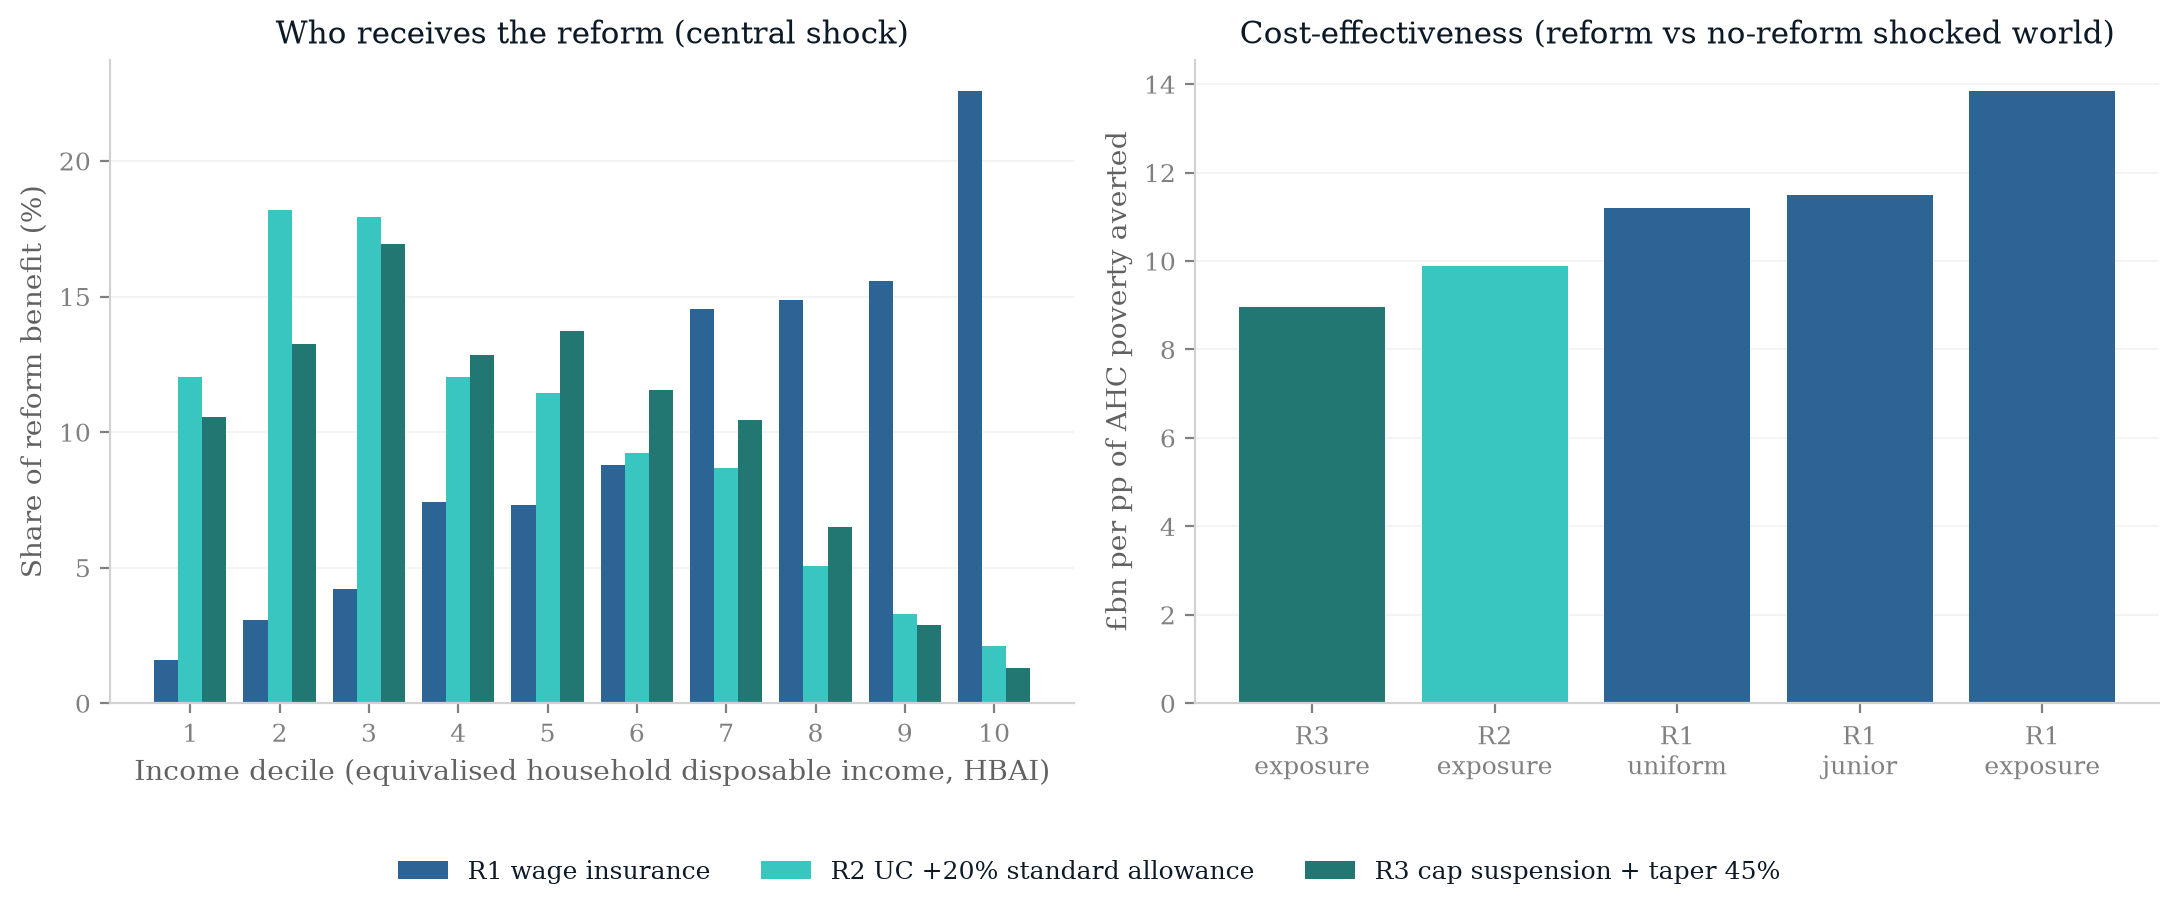
\includegraphics[width=.95\textwidth]{../results/policy/policy_reforms.png}
\caption{The three policy reforms on top of the central shock: fiscal cost, poverty and Gini effects, and the decile distribution of household gains. All panels show shocked-plus-reform minus shocked, seed 0, 2026.}
\label{fig:policy}
\end{figure}

The reform comparisons are far less sensitive to the displacement draw than the shock aggregates: over 20 Monte Carlo draws the wage-insurance cost varies by only $\pm$\pounds 0.2 billion (\pounds 21.4 $\pm$ 0.2 billion under exposure incidence, averting $1.44 \pm 0.10$ BHC points), and the UC-side instruments by less (R2: \pounds 5.69 $\pm$ 0.03 billion, $-0.54 \pm 0.02$ points; R3: \pounds 4.57 $\pm$ 0.06 billion, $-0.47 \pm 0.03$ points), so the cost-effectiveness ranking survives the draw noise comfortably. It also survives---indeed strengthens under---the six-month duration variant of Section~\ref{sec:results-aggregates}: with displaced workers recovering half a year's earnings, a duration-consistent wage insurance costs \pounds 33 $\pm$ 6 billion per BHC poverty point averted against \pounds 11.0 $\pm$ 0.6 billion for the UC uplift, because shortening the earnings loss shrinks the poverty problem faster than it shrinks the earnings-proportional transfer. Because Section~\ref{sec:results-incidence} established that incidence is the paper's central uncertainty, I re-run the wage-insurance reform under the junior-concentrated and uniform incidence families. The cost-effectiveness ranking is robust: R1 costs \pounds 14.3 billion per AHC point under junior incidence and \pounds 11.8 billion under uniform incidence, so even in its most favourable incidence world wage insurance only just reaches the \pounds 10.3--10.4 billion achieved by the UC-side instruments under the central family. The gross cost of R1 is nearly invariant across families (\pounds 20.3--21.4 billion), as it must be when the aggregate displaced wage bill is held approximately fixed; what varies is how much of that spending lands near the poverty line.

None of this settles the choice of instrument. Wage insurance addresses a different objective---consumption smoothing and earnings-loss compensation for the displaced themselves, most of whom are not poor---and a government persuaded by that objective would not be deterred by an unfavourable poverty-targeting ratio. What the exercise shows is narrower: if the criterion is poverty averted per pound in the shocked world, the existing means-tested architecture, temporarily made more generous, dominates a new earnings-linked scheme, precisely because the shock modelled here falls disproportionately on households that means tests are designed to exclude.

\subsection{The tax-composition channel}
\label{sec:policy-tax}

The reforms above spend money into a fiscal position that the shock has already damaged, and the size of that damage depends on a question the microsimulation cannot answer by itself: where does the displaced wage bill go? The OBR's recent analysis of AI-related fiscal risks \citep{obr2026} emphasises that labour displacement erodes the income-tax and National Insurance base even if aggregate output is unchanged, with the fiscal outcome hinging on how much of the lost labour income reappears as taxable profit. I price this channel on top of the microsimulation with a simple accounting exercise. Let $\phi$ denote the share of the displaced wage bill that reappears as corporate profits taxed at the 25 per cent main rate. In the central scenario the displaced wage bill is \pounds 77.9 billion and the effective income-tax-plus-NICs rate on displaced workers' earnings is 25.0 per cent, so the labour tax forgone is \pounds 19.5 billion---and because that effective labour rate almost exactly equals the corporation-tax main rate, the shortfall is very nearly $(1-\phi) \times 0.25 \times$ the displaced wage bill. At $\phi=0$ the net revenue shortfall is the microsimulation's \pounds 21.5 billion; at $\phi=0.5$ it falls to \pounds 11.8 billion; and at $\phi=1$ the labour-to-capital channel is almost exactly self-financing (a \pounds 0.03 billion surplus relative to full labour taxation), leaving only a residual \pounds 2.1 billion net cost, chiefly shock-induced benefit spending together with smaller non-labour-tax revenue changes. Figure~\ref{fig:phi} traces the full grid over displacement rates and $\phi$.

\begin{figure}[htbp]
\centering
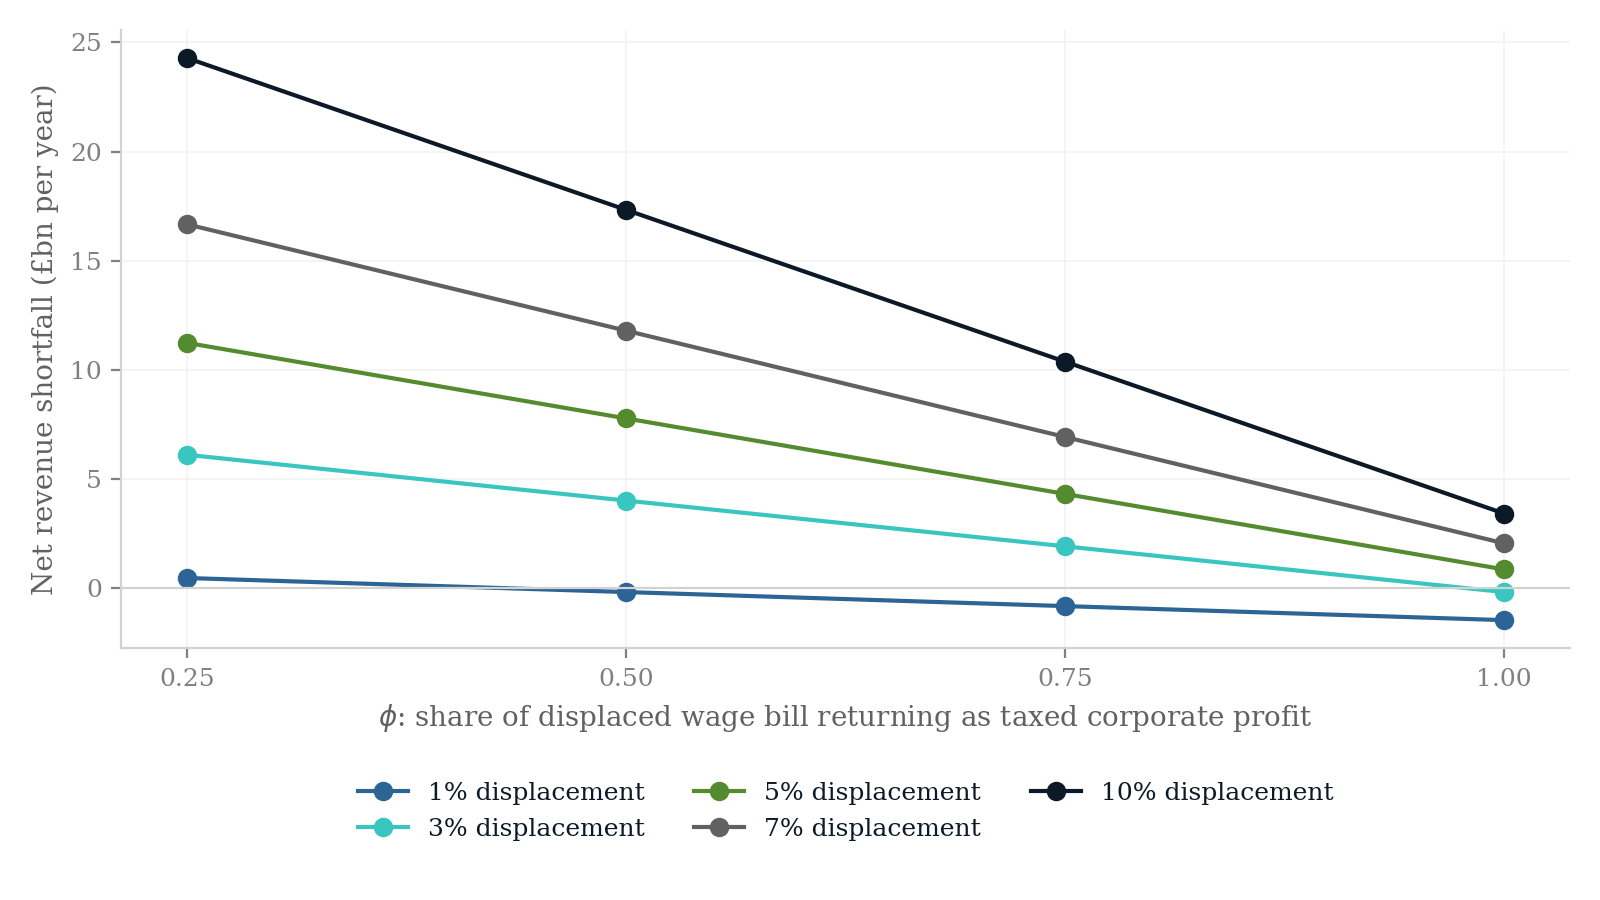
\includegraphics[width=.85\textwidth]{../results/tax_composition/revenue_shortfall_phi.png}
\caption{Net revenue change by displacement rate and $\phi$, the share of the displaced wage bill reappearing as corporate profits taxed at 25 per cent. The $\phi=0$ line is the microsimulation's net revenue change; higher $\phi$ adds recouped corporation tax outside the simulation.}
\label{fig:phi}
\end{figure}

Revenue neutrality, however, is not distributional neutrality. To see who receives the recomposed income, I simulate a dividend-recycling case at $\phi=0.5$ with a payout ratio of 0.5 (a parameter, not an estimate): \pounds 19.5 billion of post-CT profits are distributed pro rata to existing FRS dividend holders, with the dividend tax on those distributions captured inside the simulation. The result is stark. The Gini rises by a further 0.62 percentage points relative to the shocked world without recycling, and poverty---before or after housing costs---moves by exactly zero: the recycled dividends reach no household near the poverty line. The decile pattern of the gains is lumpy because FRS dividend records are sparse, but the message is not: deciles 1--4 receive exactly nothing. Even in the most fiscally benign reading of the shock, in which the Exchequer recovers essentially all of the lost labour tax through the corporate channel, the compositional shift from wages to capital income leaves the bottom of the distribution no better off and the overall distribution more unequal---which is precisely the configuration in which the transfer-side instruments of Section~\ref{sec:policy-reforms} would be needed most.

Two caveats bound this exercise. It is static accounting layered on top of the microsimulation: the incidence of corporation tax is not modelled, the corporation-tax base is assumed equal to accounting profit (no allowances, losses or profit shifting), and the effective labour rate is a pro-rata attribution of income tax and NICs to employment income that ignores the schedule ordering of savings and dividend bands. And $\phi$ itself is the free parameter the whole channel turns on; I present a grid rather than a point estimate because nothing in my framework pins it down.

\section{Discussion and policy implications}
\label{sec:discussion}

The results should be read as scenario analysis, not prediction. We do not forecast the pace or extent of AI adoption in the United Kingdom; we trace the distributional and fiscal consequences that would follow \emph{if} labour-market shocks of a given size and occupational incidence were to materialise, under tax-benefit rules as legislated. The early observational record justifies the full width of the grid, including its benign corner: population-scale Danish evidence finds minimal earnings and hours effects of chatbot adoption to date \citep{humlum2025}, and postings-based analyses disagree on whether the entry-level slowdown in exposed occupations is attributable to AI at all. UK postings evidence points to a modest relative contraction in exposed occupations since late 2022 \citep{henseke2025}, but nothing yet at the scale of our central scenario. The Office for Budget Responsibility treats AI principally as a productivity risk to its fiscal projections \citep{obr2025}; our estimates supply the complementary labour-incidence arithmetic that such projections currently leave implicit. The scenario parameters are calibration conventions transported from headline estimates in the empirical and modelling literature---including \citet{briggs2023} and \citet{cazzaniga2024}---rather than elasticities estimated on UK data, and the wide span between our mildest and harshest cells is a deliberate acknowledgement of the uncertainty surrounding all of these anchors. The incidence gradient itself is an assumption in every family we run; what the paper establishes is how the tax-benefit system mediates each assumed incidence.

Two findings organise the discussion. The first is that the UK tax-benefit system provides substantial automatic insurance to low-income households: means-tested support---principally Universal Credit---absorbs a large share of the market-income losses in the lower deciles, while progressive income taxation claws back part of the losses higher up before they reach disposable income. This cushioning is not free. In the central scenario the combined cost of lower receipts and higher benefit expenditure is \pounds 18.4~billion a year, and the cost scales with the severity of the shock. The protection households experience is purchased through a deterioration of the public finances.

The second finding is that the Gini of equivalised household disposable income rises in every one of the 66 shock-size cells and in all five incidence families (Sections~\ref{sec:results-grid} and~\ref{sec:results-incidence}), even though the market-income incidence in the exposure-proportional family is progressive---displacement risk rises monotonically with household income (Figure~\ref{fig:transition}), and average losses are largest at the top. That tension is the interesting result. Each displaced worker falls from somewhere on the earnings ladder to the bottom of it, while wage and capital gains lift those who remain; because the displaced come disproportionately from higher-income households, the shock simultaneously thins the upper-middle of the distribution and swells its lower tail. When households are re-ranked on post-shock income, as the Gini requires, dispersion increases even though decile-average losses computed at fixed baseline ranks look progressive. A similar re-ranking mechanism is documented for Ireland by \citet{doorley2026}, and it distinguishes the AI case from earlier automation waves, in which exposure fell on mid- and low-wage routine work \citep{autor2003, doorley2023automation}.

\subsection*{Policy implications: what depends on who bears the shock}

The central policy message follows from the incidence axis rather than from any single scenario. Inequality rises whichever family one assumes; what the incidence determines is whether the UK faces primarily a fiscal-resilience problem or a poverty-protection problem.

If the shock is top-loaded, as in the exposure-proportional family, the problem is chiefly fiscal. Displaced workers are drawn from occupations that pay well and are taxed heavily, so each displacement removes a large slug of income tax and National Insurance while adding comparatively little to means-tested expenditure. The Exchequer cost of the central shock is \pounds 18.4~billion under exposure-proportional incidence against \pounds 14.2~billion under uniform incidence---the same aggregate shock, roughly 30 per cent more expensive purely because of who bears it. Under top-loaded incidence the first-order policy question is revenue resilience: the UK tax base leans heavily on the taxation of labour income, and the workers most exposed are precisely those who contribute most to it. If AI additionally shifts the functional distribution of income from labour towards capital, the base that finances the cushioning we document would itself erode---a possibility that has motivated recent work on the taxation of capital in an AI-intensive economy \citep{bastani2024}. The tax-composition exercise in Section~\ref{sec:policy} turns that possibility into a quantified scenario for the Treasury: because the effective labour-tax rate on displaced earnings is almost exactly the corporation-tax main rate, the net revenue shortfall is governed by the share of the lost wage bill that reappears as taxable corporate profit---full reappearance is roughly revenue-neutral, no reappearance leaves the whole labour-tax loss uncovered, and the harm is distributional rather than fiscal, since recycled dividends raise the Gini while reaching no household near the poverty line. The exercise is static accounting on top of the microsimulation, with corporation-tax incidence not modelled, but it gives base-erosion discussions a concrete UK arithmetic to anchor on.

If instead the shock lands flatter or on junior workers, the fiscal exposure moderates but the poverty exposure does not. Uniform incidence is the cheapest family we run, yet its poverty effect (+1.83 points before housing costs) is essentially the same as the exposure family's (+1.87), and its Gini effect is the largest of the five families (+1.14 points). Junior-concentrated incidence costs slightly more than the exposure family (\pounds 19.4~billion) with a near-identical poverty effect. In these worlds the binding constraint is the adequacy of out-of-work support, and the relevant instruments are benefit levels, the contributory window, and---for the junior case---the entry prospects of young workers. Evidence that generative AI operates as a seniority-biased technology, compressing demand for junior and entry-level roles in exposed occupations \citep{hosseini2026, brynjolfsson2025}, with early UK corroboration in \citet{kleinteeselink2025}, argues for close monitoring of youth labour-market entry. Our junior-concentrated family can only re-weight who is displaced within a single year; the dynamic costs of a scarred entry cohort---foregone experience, delayed progression, persistent earnings losses---lie outside a static framework, so even that family understates the long-run burden on new entrants.

The fiscal-versus-poverty framing also now has a policy answer rather than only a diagnosis. The counterfactual reforms in Section~\ref{sec:policy} show that temporary Universal-Credit-side stabilisers---a circuit-breaker uplift to the standard allowance, or a benefit-cap suspension combined with a taper cut---deliver a point of after-housing-costs poverty reduction at roughly \pounds 10~billion, against \pounds 13--14~billion for an earnings-linked wage-insurance scheme, because wage insurance is earnings-proportional and much of its benefit accrues in the upper half of the baseline distribution. Wage insurance buys more total poverty reduction, but at disproportionate cost; a government facing a top-loaded shock and a strained revenue base gets more protection per pound by working through the existing means-tested architecture than by building an earnings-replacement scheme alongside it.

The expertise-compression family, our stylised stress test of the view that AI erodes the returns to accumulated expertise, is the worst of both worlds among the stylised families: the most expensive (\pounds 24.5~billion) and the most poverty-raising (+2.12 points) of the four---and the measured family exceeds it on both margins (Table~\ref{tab:incidence}). If that view proves correct, neither fiscal buffers nor poverty protection alone suffices; both margins bind at once.

The shock also has a geography, and it does not track existing regional-policy maps. In the constituency analysis of Section~\ref{sec:results-geo}, the largest proportionate income losses fall on Northern Ireland---the worst-hit region, at $-2.3$ per cent of aggregate household income---and Scotland, while Wales and the South East are mildest; the hardest-hit constituencies mix Northern Irish seats with inner-London ones. An AI labour shock is not a rerun of deindustrialisation: because exposure follows clerical and professional employment, it strikes administrative and professional centres wherever they sit, and a levelling-up strategy calibrated to the geography of manufacturing decline would miss much of it. These geographic results rest on imputed occupations on the enhanced 2023--24 dataset (Appendix~\ref{app:geo-imputation}) and are indicative of relative, not absolute, local impacts.

Two implications hold across all families. First, because the modelled losses fall on identifiable occupational groups rather than diffusely across the workforce, retraining and lifelong-learning provision targeted at exposed occupations is the most direct lever available; the tax-benefit system can replace income but cannot restore occupational attachment. Second, since measured inequality rises under every incidence we examine, distributional monitoring should not wait for evidence on which incidence is materialising: the direction of the inequality effect is not in doubt within this framework, only its composition.

Taken together, the results suggest that the United Kingdom would enter a period of AI-driven labour-market disruption with a tax-benefit system that redistributes the losses effectively but does not, and cannot, prevent them. The system converts each market-income shock into a smaller disposable-income shock at a substantial, incidence-dependent fiscal cost, while the polarising character of displacement pushes measured inequality upwards regardless of who bears it. Policy attention is best directed at the margins the system does not reach: the occupational reallocation of exposed workers, the entry prospects of the young, and the robustness of a labour-taxation-heavy revenue base.

\section{Limitations and further work}
\label{sec:limitations}

Several limitations qualify the results. We state them plainly, together with the measurement conventions a reader needs in order to compare our figures with official statistics.

\paragraph{Measurement conventions.} All income results are on the HBAI cash disposable income concept at the household level, equivalised; poverty and inequality statistics share that concept. In computing the Gini we bottom-code negative equivalised incomes at zero. Our baseline Gini is 0.309, below the official UK figure of roughly 0.34, because we use the plain Family Resources Survey without the SPI adjustment that corrects for under-coverage of top incomes; levels should therefore not be compared directly with official statistics, though changes---the objects of interest---are computed on a consistent basis throughout.

\paragraph{Monte Carlo conventions.} Which results rest on which random draws matters for interpretation; the conventions are set out in Section~\ref{sec:microsim} and Appendix~\ref{app:seeds}. Single-draw figures carry draw noise that the averaged figures do not, although the 20-draw runs indicate the aggregate magnitudes are stable across seeds.

\paragraph{Exposure resolution and crosswalk provenance.} Occupational exposure is assigned at the 1-digit SOC level, because the Family Resources Survey records occupation only at the major-group level; within-group heterogeneity in AI exposure---substantial in the indices of \citet{felten2021}, \citet{webb2019} and \citet{eloundou2023}---is averaged away. The exposure scores themselves reach the FRS through a reconstructed pipeline: the complementarity adjustment is rebuilt from published sources (recovering the published ranking up to a level offset), and the US occupational scores are carried to SOC2020 through a chained SOC2018--SOC2010--ISCO--SOC2020 crosswalk with ASHE employment weights available for 340 of 412 unit groups. A UK-native task-based index (GAISI) built from British Skills and Employment Survey data now exists \citep{henseke2025}; adopting it, together with an imputation of detailed occupation from the Labour Force Survey, would remove the crosswalk and the resolution constraint at once, and is the first item on our agenda.

\paragraph{Survey weights.} We use the uncalibrated FRS grossing weights rather than PolicyEngine's enhanced dataset. The enhanced dataset improves aggregate fiscal accuracy through reweighting and household cloning, but cloning breaks the one-to-one correspondence between records and observed occupations on which the exposure join depends. Aggregate fiscal magnitudes should be read with the usual caveats attaching to unadjusted survey grossing.

\paragraph{Static displacement.} Displaced workers are fully out of work in the simulated year---earnings, hours, employee pension contributions and salary sacrifice set to zero, no statutory pay, benefit entitlements recomputed under existing rules---while dual jobholders retain self-employment income. The duration structure of unemployment is not modelled, so the exhaustion of contributory benefits (new-style Jobseeker's Allowance is payable for at most six months) cannot be expressed; over longer horizons we overstate the support available to displaced workers without means-tested entitlements.

\paragraph{The capital channel.} The capital-income measure covers only interest and dividends, excluding rental income and returns inside private pensions, and household surveys under-represent top incomes and capital income in particular. The concentration of capital income in the top decile that drives this channel is, if anything, understated. Linked administrative or wealth-survey data (the Wealth and Assets Survey) would sharpen it considerably.

\paragraph{The self-employed.} All shock scenarios exclude the self-employed. Exposure indices and the displacement literature underpinning our parameters are defined over employees, and self-employed earnings dynamics under AI adoption may include both displacement and new opportunities; we exclude the group rather than impose an arbitrary treatment. Since self-employment is a meaningful share of UK employment and is concentrated in some exposed occupations, this is a substantive omission.

\paragraph{Mechanisms and anchors.} Where we attribute decile-level patterns to particular mechanisms---the thinness of savings buffers at the bottom, income pooling within couples---these attributions are hypotheses consistent with the data rather than results of a formal decomposition, and we flag them as such. The scenario anchors, likewise, are author-designed stress tests transported from headline estimates: the 1 per cent ``low'' cell is a sensitivity case rather than an employment estimate, the 7 per cent displacement and 2.6 per cent wage figures are conventions converting task-exposure and productivity estimates into single-year shocks, and the paper-anchored scenarios are transpositions, not implementations, of the studies they draw on. As UK-specific evidence accumulates---early examples include \citet{kleinteeselink2025} and \citet{rockall2025}---the scenarios can be re-anchored, and the gap between scenario analysis and conditional forecast will narrow. Extending the exposure measurement, restoring calibrated weights through an occupation-preserving reweighting, and introducing benefit-duration dynamics are the immediate priorities for further work.


\clearpage
\begin{thebibliography}{99}

\bibitem[Acemoglu(2025)]{acemoglu2025}
Acemoglu, D. (2025).
\newblock The simple macroeconomics of AI.
\newblock \emph{Economic Policy}, 40(121), 13--58.

\bibitem[Acemoglu and Restrepo(2018)]{acemoglu2018}
Acemoglu, D. and Restrepo, P. (2018).
\newblock The race between man and machine: Implications of technology for growth, factor shares, and employment.
\newblock \emph{American Economic Review}, 108(6), 1488--1542.

\bibitem[Acemoglu and Restrepo(2022)]{acemoglu2022tasks}
Acemoglu, D. and Restrepo, P. (2022).
\newblock Tasks, automation, and the rise in US wage inequality.
\newblock \emph{Econometrica}, 90(5), 1973--2016.

\bibitem[Acemoglu et~al.(2022)]{acemoglu2022vacancies}
Acemoglu, D., Autor, D., Hazell, J. and Restrepo, P. (2022).
\newblock Artificial intelligence and jobs: Evidence from online vacancies.
\newblock \emph{Journal of Labor Economics}, 40(S1), S293--S340.

\bibitem[Agrawal et~al.(2018)]{agrawal2018}
Agrawal, A., Gans, J. and Goldfarb, A. (2018).
\newblock \emph{Prediction Machines: The Simple Economics of Artificial Intelligence}.
\newblock Harvard Business Review Press, Boston, MA.

\bibitem[Autor et~al.(2003)]{autor2003}
Autor, D.~H., Levy, F. and Murnane, R.~J. (2003).
\newblock The skill content of recent technological change: An empirical exploration.
\newblock \emph{The Quarterly Journal of Economics}, 118(4), 1279--1333.

\bibitem[Autor(2024)]{autor2024}
Autor, D. (2024).
\newblock Applying AI to rebuild middle class jobs.
\newblock NBER Working Paper No.~32140, National Bureau of Economic Research, Cambridge, MA.

\bibitem[Bastani and Waldenstr\"{o}m(2024)]{bastani2024}
Bastani, S. and Waldenstr\"{o}m, D. (2024).
\newblock AI, automation and taxation.
\newblock CESifo Working Paper No.~11084 / IZA Policy Paper No.~212, Munich and Bonn.

\bibitem[Briggs and Kodnani(2023)]{briggs2023}
Briggs, J. and Kodnani, D. (2023).
\newblock The potentially large effects of artificial intelligence on economic growth.
\newblock Goldman Sachs Global Economics Analyst, Goldman Sachs.

\bibitem[Brynjolfsson et~al.(2025a)]{brynjolfsson2025}
Brynjolfsson, E., Chandar, B. and Chen, R. (2025a).
\newblock Canaries in the coal mine? Six facts about the recent employment effects of artificial intelligence.
\newblock Working paper, Stanford Digital Economy Lab.

\bibitem[Brynjolfsson et~al.(2025b)]{brynjolfsson2025qje}
Brynjolfsson, E., Li, D. and Raymond, L. (2025b).
\newblock Generative AI at work.
\newblock \emph{The Quarterly Journal of Economics}, 140(2), 889--942.

\bibitem[Cazzaniga et~al.(2024)]{cazzaniga2024}
Cazzaniga, M., Jaumotte, F., Li, L., Melina, G., Panton, A.~J., Pizzinelli, C., Rockall, E. and Tavares, M.~M. (2024).
\newblock Gen-AI: Artificial intelligence and the future of work.
\newblock IMF Staff Discussion Note SDN/2024/001, International Monetary Fund, Washington, DC.

\bibitem[Doorley et~al.(2023)]{doorley2023automation}
Doorley, K., Gromadzki, J., Lewandowski, P., Tuda, D. and Van~Kerm, P. (2023).
\newblock Automation and income inequality in Europe.
\newblock IZA Discussion Paper No.~16499, Institute of Labor Economics, Bonn.

\bibitem[Doorley et~al.(2026)]{doorley2026}
Doorley, K., O'Connor, S., O'Shea, R. and Tuda, D. (2026).
\newblock Artificial intelligence and income inequality in Ireland.
\newblock Jointly-published Report 16, Economic and Social Research Institute and Department of Finance, Dublin.

\bibitem[DSIT and DfE(2023)]{dsit2023}
Department for Science, Innovation and Technology and Department for Education (2023).
\newblock The impact of AI on UK jobs and training.
\newblock UK Government, London.

\bibitem[Eloundou et~al.(2024)]{eloundou2023}
Eloundou, T., Manning, S., Mishkin, P. and Rock, D. (2024).
\newblock GPTs are GPTs: Labor market impact potential of LLMs.
\newblock \emph{Science}, 384(6702), 1306--1308.

\bibitem[Felten et~al.(2021)]{felten2021}
Felten, E., Raj, M. and Seamans, R. (2021).
\newblock Occupational, industry, and geographic exposure to artificial intelligence: A novel dataset and its potential uses.
\newblock \emph{Strategic Management Journal}, 42(12), 2195--2217.

\bibitem[Frey and Osborne(2017)]{frey2017}
Frey, C.~B. and Osborne, M.~A. (2017).
\newblock The future of employment: How susceptible are jobs to computerisation?
\newblock \emph{Technological Forecasting and Social Change}, 114, 254--280.

\bibitem[Goos and Manning(2007)]{goosmanning2007}
Goos, M. and Manning, A. (2007).
\newblock Lousy and lovely jobs: The rising polarization of work in Britain.
\newblock \emph{The Review of Economics and Statistics}, 89(1), 118--133.

\bibitem[Goos et~al.(2014)]{goos2014}
Goos, M., Manning, A. and Salomons, A. (2014).
\newblock Explaining job polarization: Routine-biased technological change and offshoring.
\newblock \emph{American Economic Review}, 104(8), 2509--2526.

\bibitem[Henseke et~al.(2025)]{henseke2025}
Henseke, G. et al. (2025).
\newblock How exposed are UK jobs to generative AI? The GAISI index.
\newblock arXiv:2507.22748.

\bibitem[Hosseini and Lichtinger(2026)]{hosseini2026}
Hosseini, S. and Lichtinger, G. (2026).
\newblock Generative AI as seniority-biased technological change: Evidence from U.S. r\'{e}sum\'{e} and job posting data.
\newblock SSRN Working Paper No.~5425555.

\bibitem[Humlum and Vestergaard(2025)]{humlum2025}
Humlum, A. and Vestergaard, E. (2025).
\newblock Large language models, small labor market effects.
\newblock Working paper, University of Chicago Becker Friedman Institute.

\bibitem[ILO(2025)]{ilo2025}
International Labour Organization (2025).
\newblock Generative AI and jobs: A 2025 update.
\newblock ILO, Geneva.

\bibitem[Klein~Teeselink(2025)]{kleinteeselink2025}
Klein~Teeselink, B. (2025).
\newblock Generative AI and labor market outcomes: Evidence from the UK.
\newblock SSRN Working Paper No.~5516798.

\bibitem[Korinek and Stiglitz(2019)]{korinek2019}
Korinek, A. and Stiglitz, J.~E. (2019).
\newblock Artificial intelligence and its implications for income distribution and unemployment.
\newblock In Agrawal, A., Gans, J. and Goldfarb, A. (eds), \emph{The Economics of Artificial Intelligence: An Agenda}, University of Chicago Press, Chicago, 349--390.

\bibitem[Moll et~al.(2022)]{moll2022}
Moll, B., Rachel, L. and Restrepo, P. (2022).
\newblock Uneven growth: Automation's impact on income and wealth inequality.
\newblock \emph{Econometrica}, 90(6), 2645--2683.

\bibitem[Noy and Zhang(2023)]{noy2023}
Noy, S. and Zhang, W. (2023).
\newblock Experimental evidence on the productivity effects of generative artificial intelligence.
\newblock \emph{Science}, 381(6654), 187--192.

\bibitem[OBR(2025)]{obr2025}
Office for Budget Responsibility (2025).
\newblock Fiscal risks and sustainability report.
\newblock OBR, London.

\bibitem[Pizzinelli et~al.(2023)]{pizzinelli2023}
Pizzinelli, C., Panton, A.~J., Tavares, M.~M., Cazzaniga, M. and Li, L. (2023).
\newblock Labor market exposure to AI: Cross-country differences and distributional implications.
\newblock IMF Working Paper WP/23/216, International Monetary Fund, Washington, DC.

\bibitem[Rockall et~al.(2025)]{rockall2025}
Rockall, E., Pizzinelli, C. and Tavares, M.~M. (2025).
\newblock Artificial intelligence and wage inequality in the United Kingdom.
\newblock IMF Working Paper, International Monetary Fund, Washington, DC.

\bibitem[Tolan et~al.(2021)]{tolan2021}
Tolan, S., Pesole, A., Mart\'{i}nez-Plumed, F., Fern\'{a}ndez-Mac\'{i}as, E., Hern\'{a}ndez-Orallo, J. and G\'{o}mez, E. (2021).
\newblock Measuring the occupational impact of AI: Tasks, cognitive abilities and AI benchmarks.
\newblock \emph{Journal of Artificial Intelligence Research}, 71, 191--236.

\bibitem[Webb(2019)]{webb2019}
Webb, M. (2019).
\newblock The impact of artificial intelligence on the labor market.
\newblock Working paper, Stanford University.

\bibitem[Williamson et~al.(2025)]{williamson2024}
Williamson, S., et~al. (2025).
\newblock Applying the complementarity-adjusted AI occupational exposure index to the United Kingdom and Ireland.
\newblock \emph{Journal for Labour Market Research}, 59, 30.

\end{thebibliography}

\clearpage
\appendix
\section{Additional tables and figures}
\label{sec:appendix}

\subsection{Seed and draw conventions}
\label{app:seeds}

Displacement is a random draw of which exposed workers lose employment,
subject to occupation-group quotas proportional to employment times mean
exposure. Throughout the paper, three conventions apply. The scenario grid
(Figures~\ref{fig:griddisp}--\ref{fig:gridgini}, and their appendix
variants below), the decomposition in Figure~\ref{fig:decomp}, the preset
scenarios and the four incidence families are single draws at seed~0. The
decile transition and wage-gain profiles (Figures~\ref{fig:transition}
and~\ref{fig:wages}) are means over 50 independent draws. The robustness
summary and the confidence intervals in Figure~\ref{fig:decomp-ci} are
20-draw Monte Carlo runs, with $\pm$ values reported as standard deviations
across draws. Within each draw, ordering keys are uniform within occupation
group, so a record's inclusion probability does not depend on its grossing
weight.

\subsection{Job loss by occupation group}

Table~\ref{tab:jobloss} reports the central-scenario displacement rate for
each SOC2020 major group. The allocation rule concentrates losses in
administrative and secretarial work (10.5 per cent of the group's
employment), managerial and professional occupations (around 9.5 per cent)
and associate professional roles, while elementary occupations---the
least-exposed group, whose normalised exposure score is zero---experience
no displacement at all. Clerical and professional work bears the shock;
manual and elementary work is insulated.

\begin{table}[htbp]
\centering
\caption{Central-scenario job loss by SOC2020 major group}
\label{tab:jobloss}
\begin{tabular}{lrrr}
\toprule
Major group & C-AIOE & Employment (m) & Job loss (\%) \\
\midrule
1 Managers, directors and senior officials & 0.62 & 2.45 & 9.6 \\
2 Professional occupations & 0.60 & 6.46 & 9.5 \\
3 Associate professional occupations & 0.47 & 3.13 & 8.5 \\
4 Administrative and secretarial occupations & 0.74 & 2.35 & 10.5 \\
5 Skilled trades occupations & $-0.33$ & 1.56 & 2.8 \\
6 Caring, leisure and other service occupations & $-0.14$ & 2.32 & 3.9 \\
7 Sales and customer service occupations & 0.27 & 1.22 & 7.2 \\
8 Process, plant and machine operatives & $-0.54$ & 1.41 & 1.3 \\
9 Elementary occupations & $-0.73$ & 2.05 & 0.0 \\
\bottomrule
\end{tabular}

\vspace{2pt}
{\footnotesize C-AIOE is the standardised complementarity-adjusted exposure
score before the min-zero normalisation used in the allocation rule.
Employment and job-loss rates are survey-weighted; single draw, seed 0.}
\end{table}

\subsection{Where the shock lands: baseline distributions}

Figures~\ref{fig:b-market}--\ref{fig:b-disposable} show the baseline
household-level decile distributions of the income components through which
the three channels operate (aggregate \pounds billion per year by decile of
equivalised household disposable income). Market income excluding capital
(\pounds 1{,}313 billion in total) and income tax and National Insurance
(\pounds 312 billion) are heavily concentrated in the top deciles---which
is why displacement of high earners is fiscally expensive. Benefits
(\pounds 320 billion) are spread across the lower and middle deciles,
peaking in deciles~3 to~5. Capital income (\pounds 23 billion of interest
and dividends) is the most concentrated series of all: the top decile
holds more than a third of the total.

\begin{figure}[htbp]
\centering
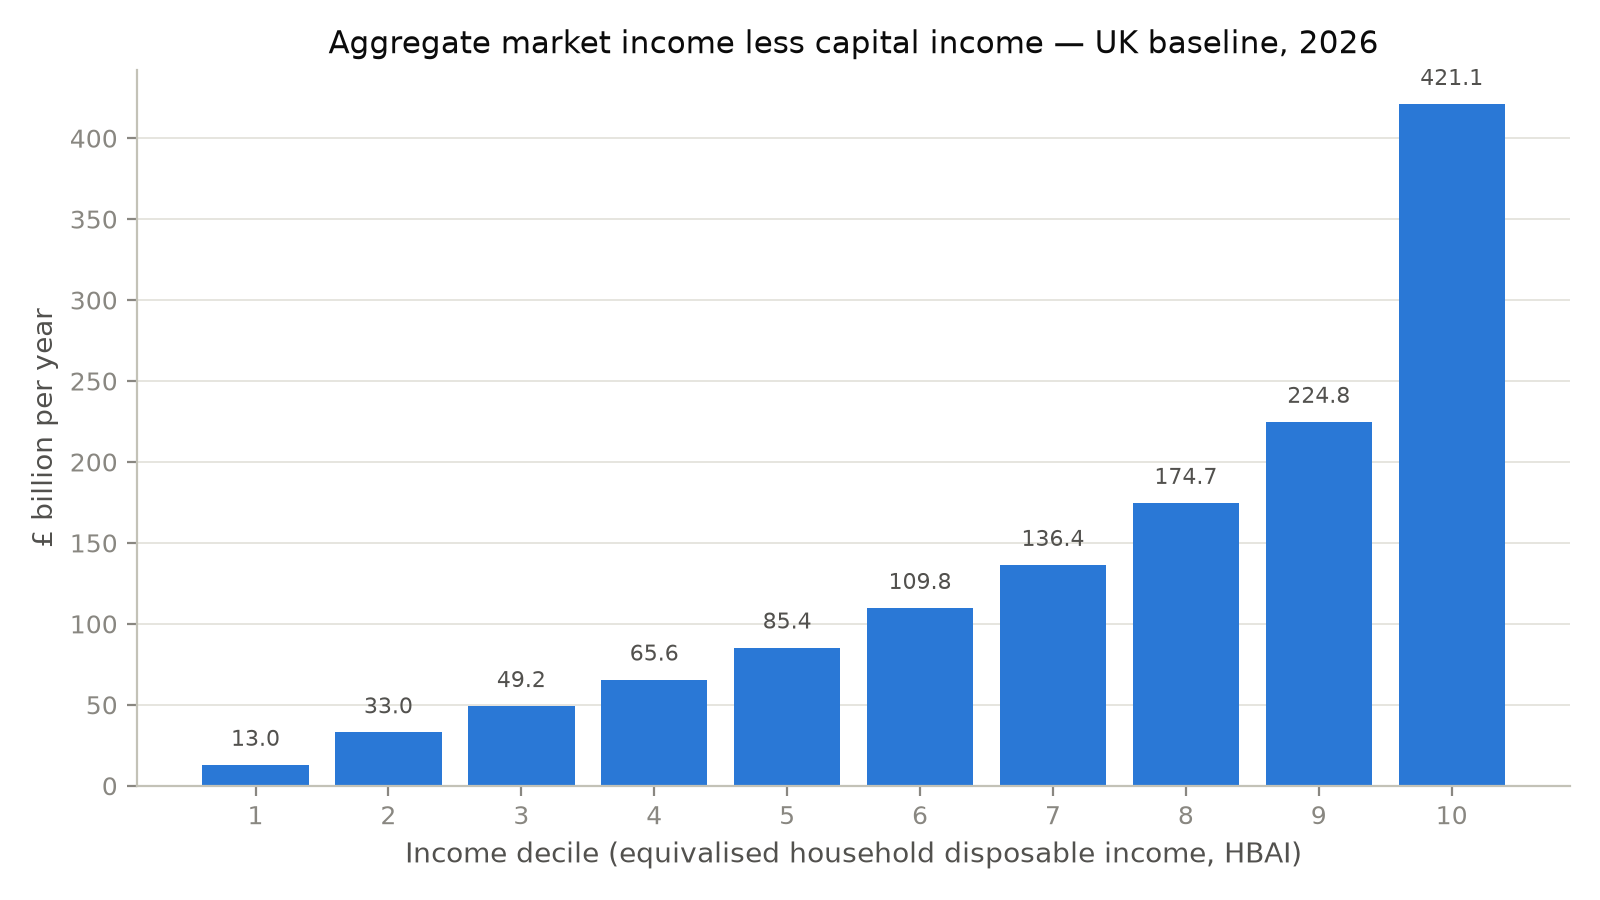
\includegraphics[width=.75\textwidth]{../results/appendix/b1_market_income_less_capital.png}
\caption{Baseline aggregate household market income (less capital income) by decile.}
\label{fig:b-market}
\end{figure}

\begin{figure}[htbp]
\centering
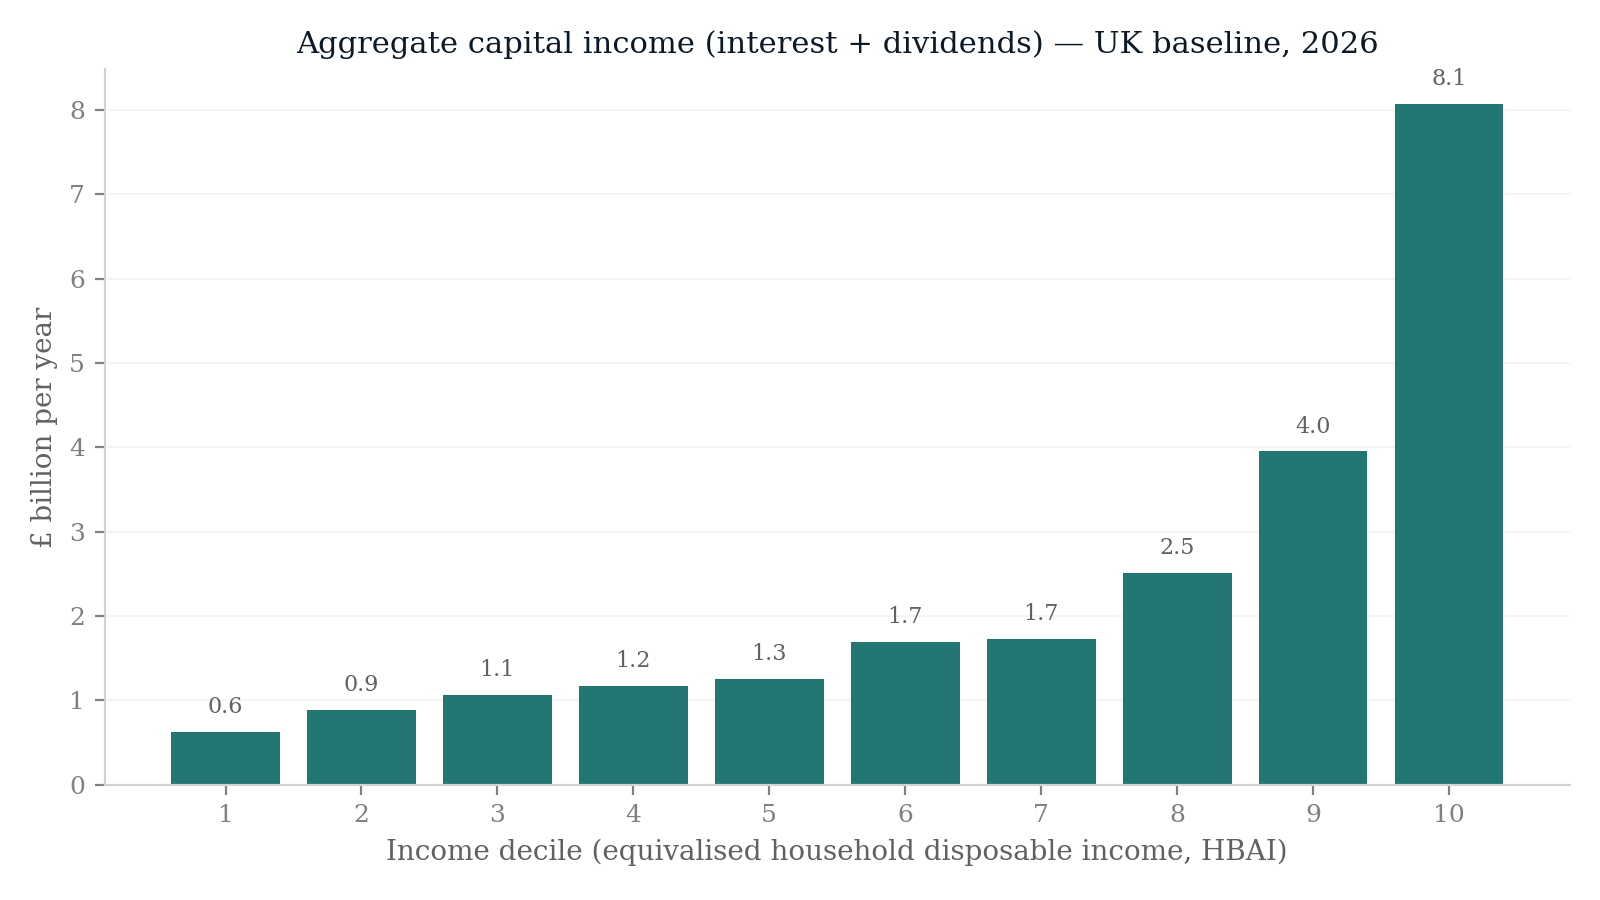
\includegraphics[width=.75\textwidth]{../results/appendix/b2_capital_income.png}
\caption{Baseline aggregate household capital income (interest and dividends) by decile.}
\label{fig:b-capital}
\end{figure}

\begin{figure}[htbp]
\centering
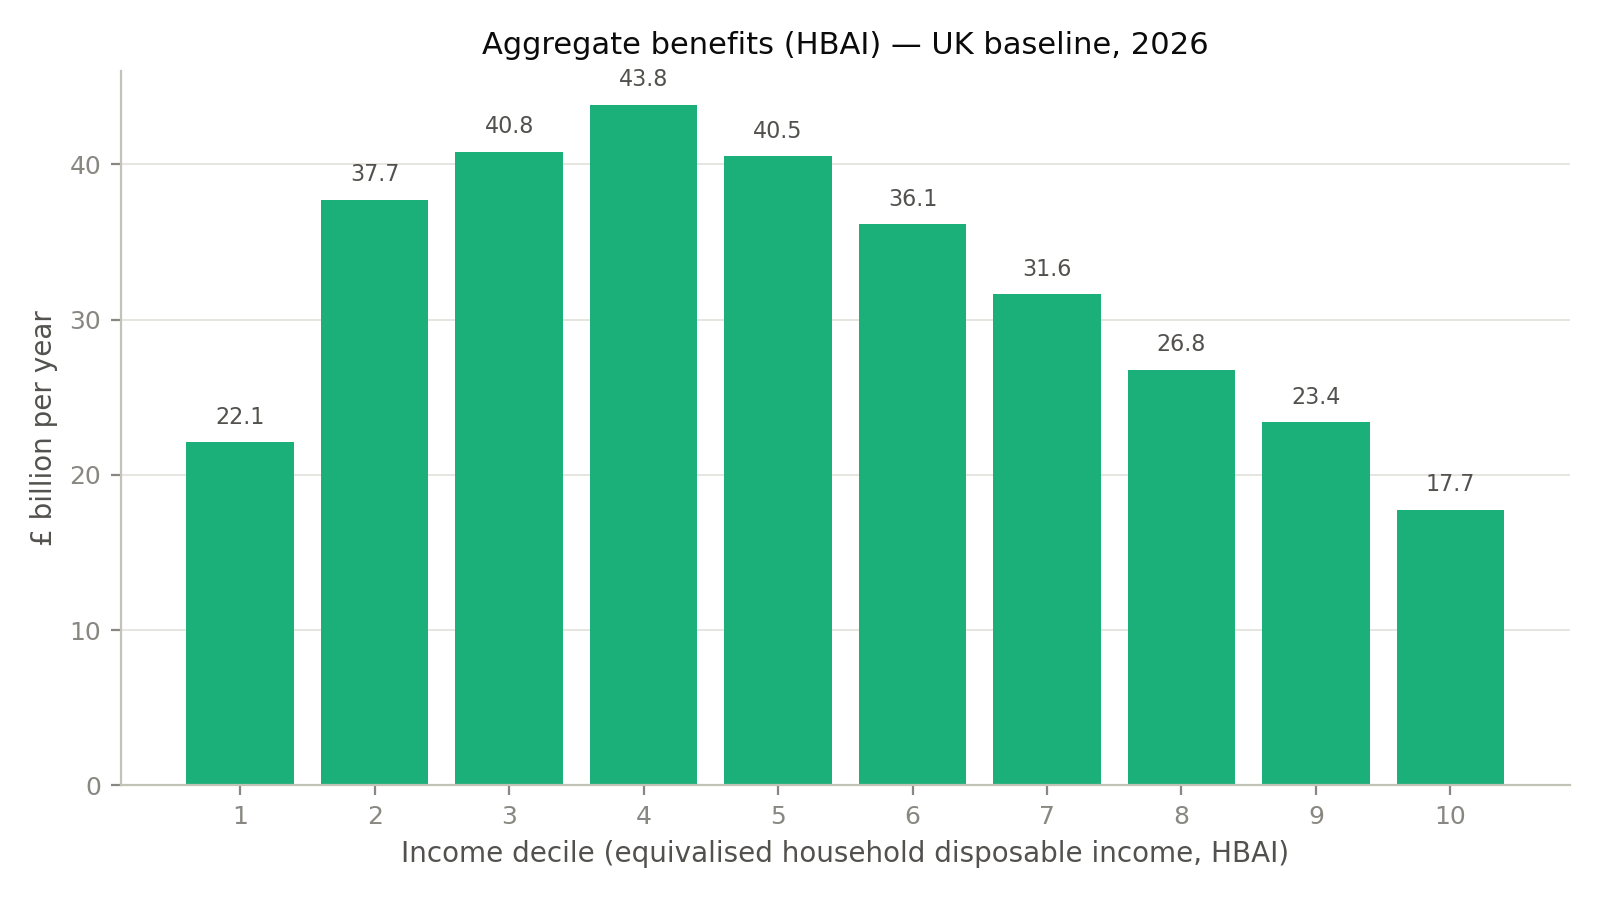
\includegraphics[width=.75\textwidth]{../results/appendix/b3_benefits.png}
\caption{Baseline aggregate household benefits by decile.}
\label{fig:b-benefits}
\end{figure}

\begin{figure}[htbp]
\centering
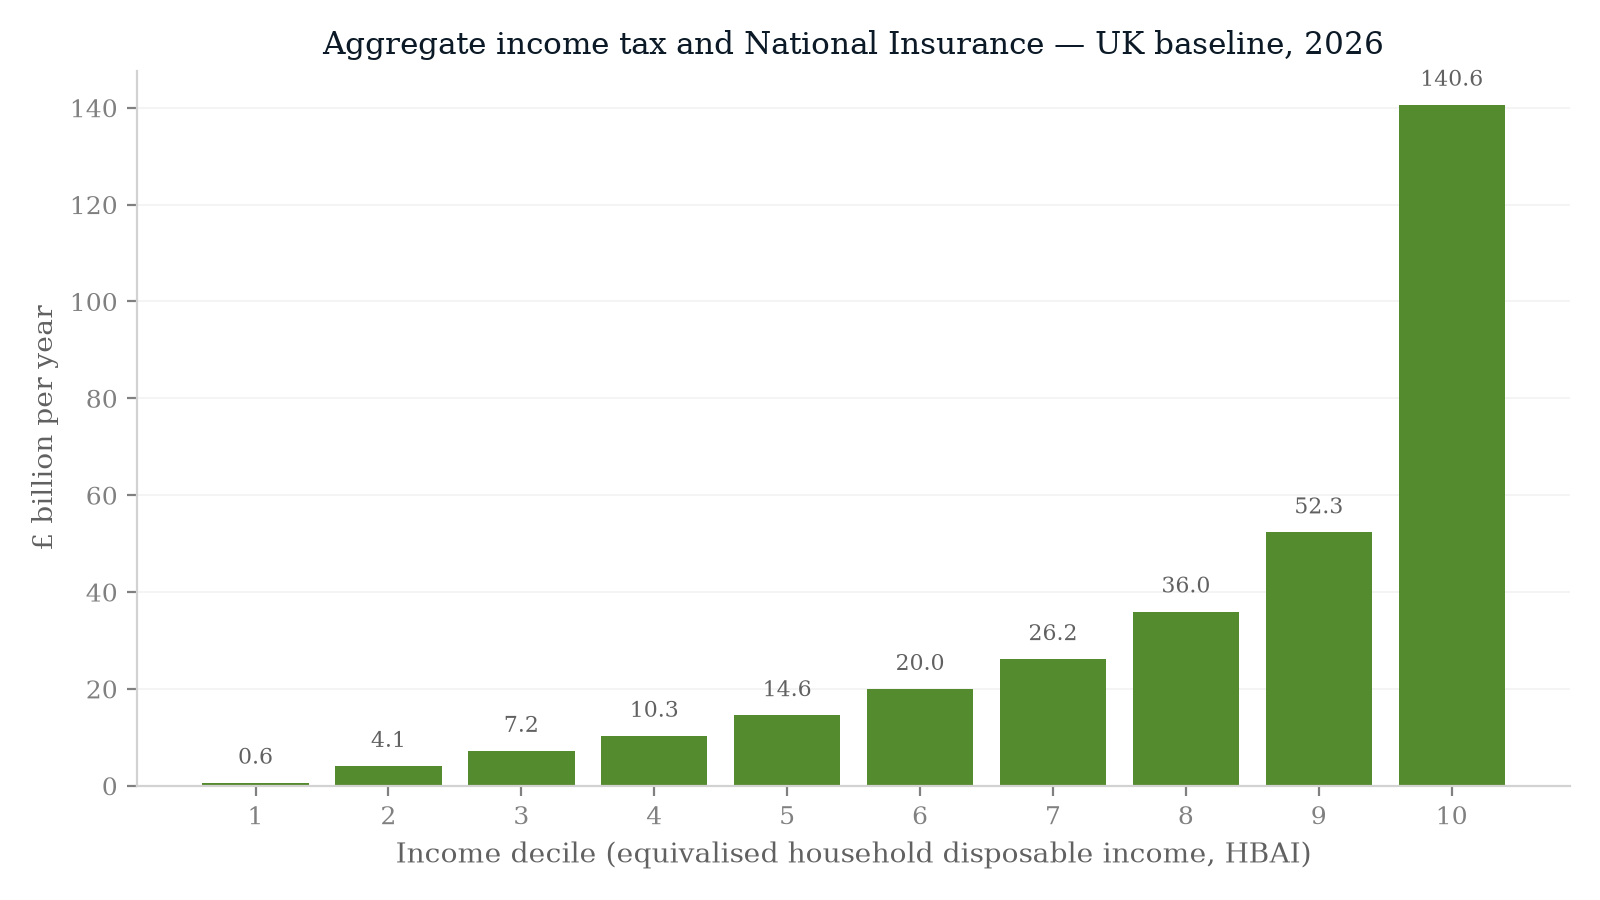
\includegraphics[width=.75\textwidth]{../results/appendix/b4_tax_and_ni.png}
\caption{Baseline aggregate household income tax and National Insurance by decile.}
\label{fig:b-tax}
\end{figure}

\begin{figure}[htbp]
\centering
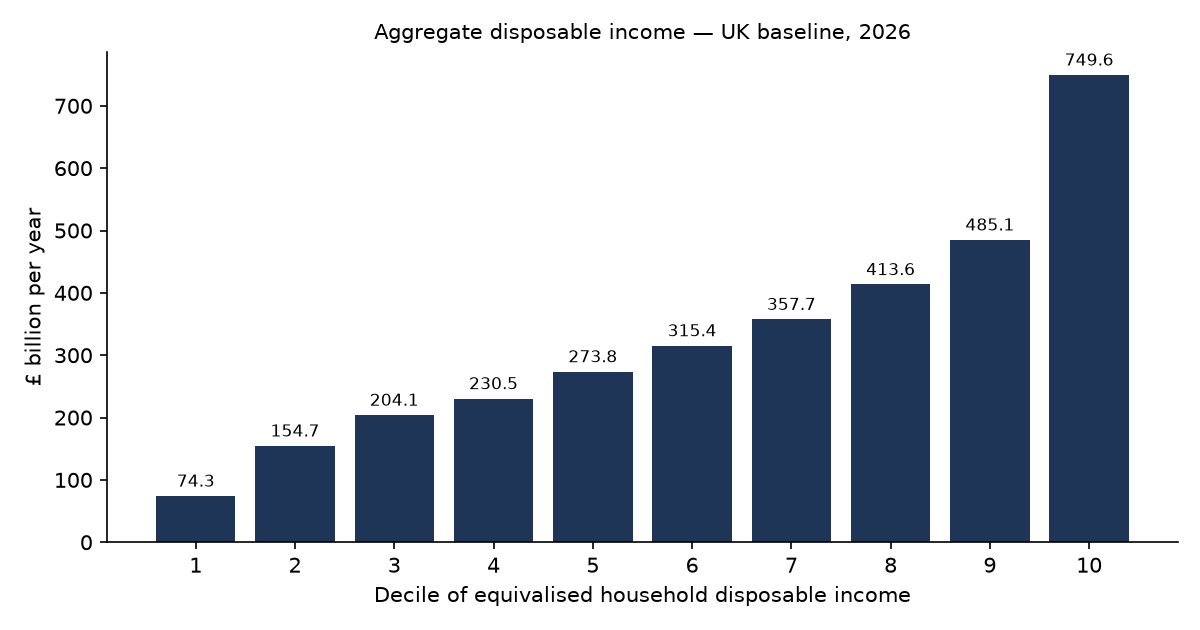
\includegraphics[width=.75\textwidth]{../results/appendix/b5_disposable_income.png}
\caption{Baseline aggregate household disposable income (HBAI concept) by decile.}
\label{fig:b-disposable}
\end{figure}

\subsection{Exposure incidence before any simulation}

Figures~\ref{fig:exp-incidence} and \ref{fig:comp-incidence} show, without
any shock, how workers in each income decile distribute across
employment-weighted tertiles of AI exposure and of complementarity. The
share of workers in the top exposure tertile rises steadily with household
income, while complementarity shows no comparable gradient---the
descriptive facts that generate the simulated incidence in
Section~\ref{sec:results}.

\begin{figure}[htbp]
\centering
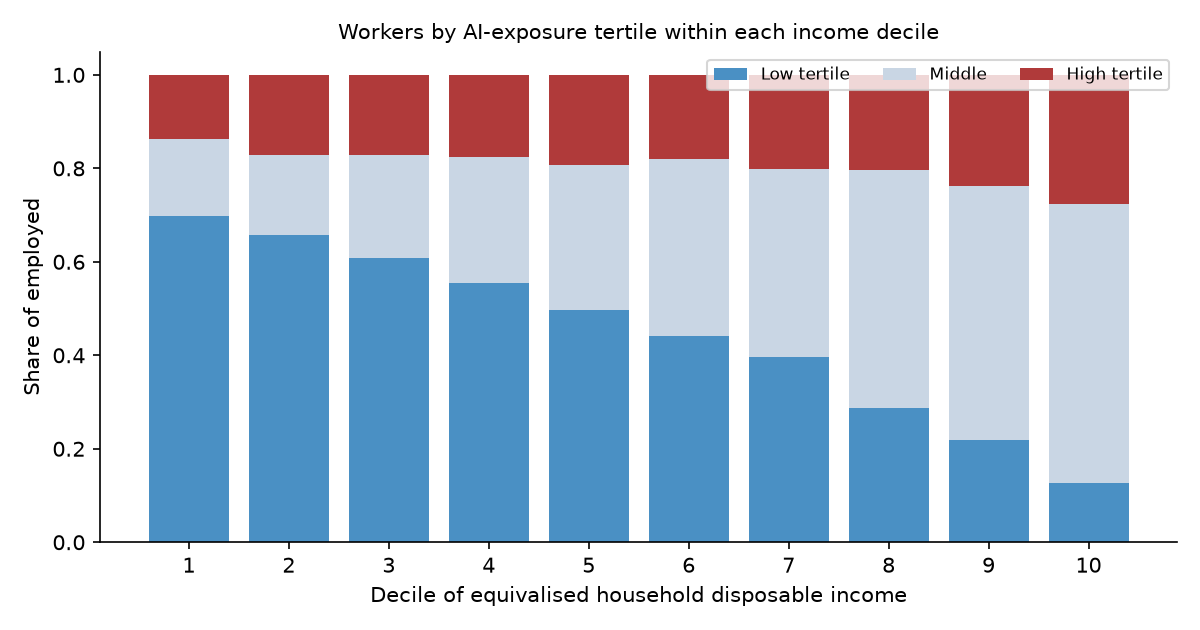
\includegraphics[width=.8\textwidth]{../results/appendix/exposure_incidence_by_decile.png}
\caption{Distribution of employed persons across AI-exposure tertiles, by income decile.}
\label{fig:exp-incidence}
\end{figure}

\begin{figure}[htbp]
\centering
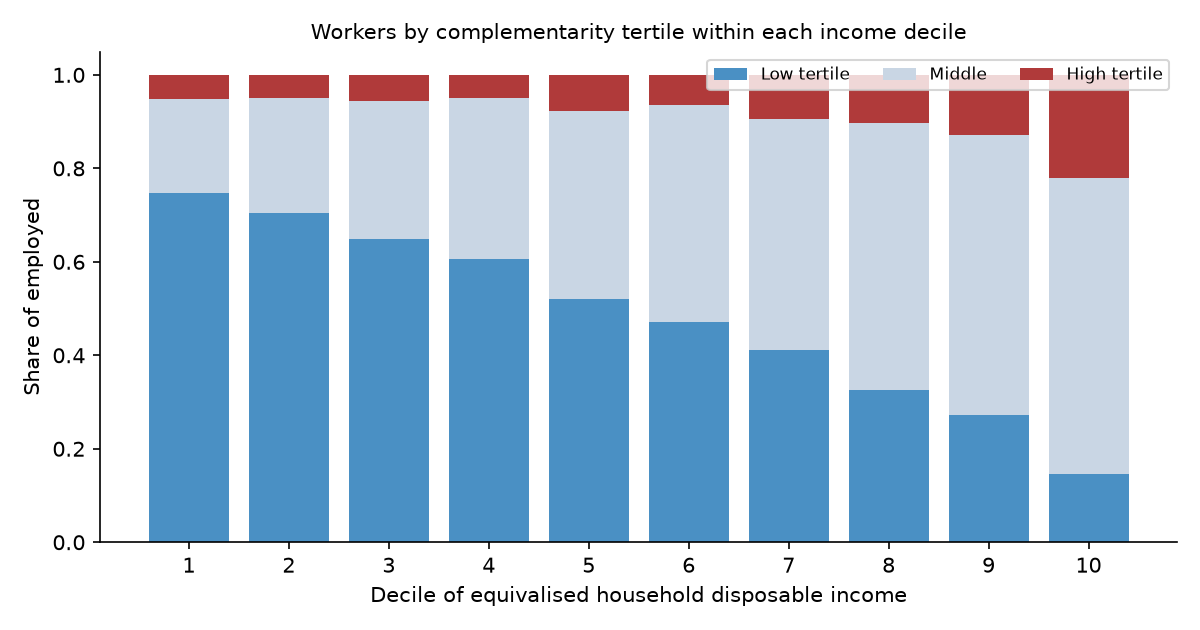
\includegraphics[width=.8\textwidth]{../results/appendix/complementarity_incidence_by_decile.png}
\caption{Distribution of employed persons across complementarity tertiles, by income decile.}
\label{fig:comp-incidence}
\end{figure}

\subsection{Monte Carlo uncertainty on the decile profile}

Figure~\ref{fig:decomp-ci} reports the central-scenario disposable-income
change by decile as the mean over twenty independent displacement draws
with 95 per cent confidence intervals. The gradient runs from $-0.5$ per
cent in the bottom decile to $-4.1$ per cent in the top. It is not quite
monotone: deciles~2 and~3 show a small reversal ($-0.88$ against $-0.82$
per cent), well inside the draw noise. The overall upward slope of the loss
profile survives the uncertainty comfortably.

\begin{figure}[htbp]
\centering
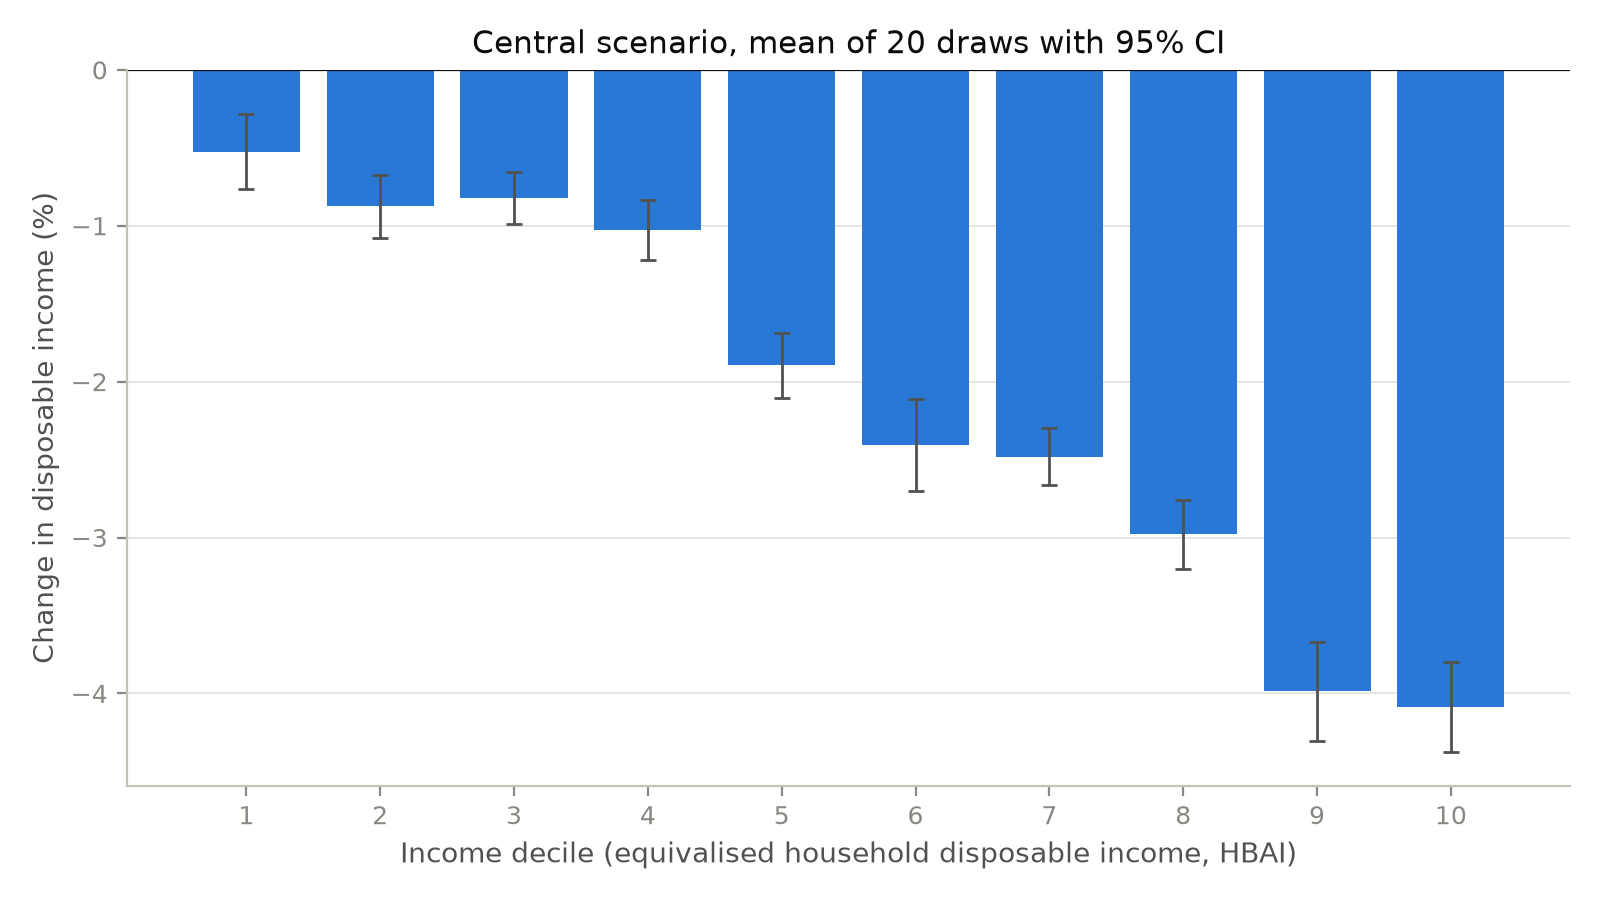
\includegraphics[width=.8\textwidth]{../results/appendix/decomposition_ci.png}
\caption{Disposable income change by decile, central scenario: mean of 20 displacement draws with 95 per cent confidence intervals.}
\label{fig:decomp-ci}
\end{figure}

\subsection{Uniform-shock and alternative-index comparisons by decile}

Figure~\ref{fig:b7} compares the central scenario against the same
aggregate shocks allocated uniformly across occupations, decile by decile;
Figure~\ref{fig:b8} repeats the central scenario with the
\citet{eloundou2023} GPT-exposure index in place of the C-AIOE. The
exposure-based allocation shifts losses up the distribution relative to a
uniform shock (top-decile losses of 3.9 against 3.0 per cent; bottom-decile
losses of 0.5 against 0.9 per cent), and the choice of exposure index
leaves the decile profile essentially unchanged.

\begin{figure}[htbp]
\centering
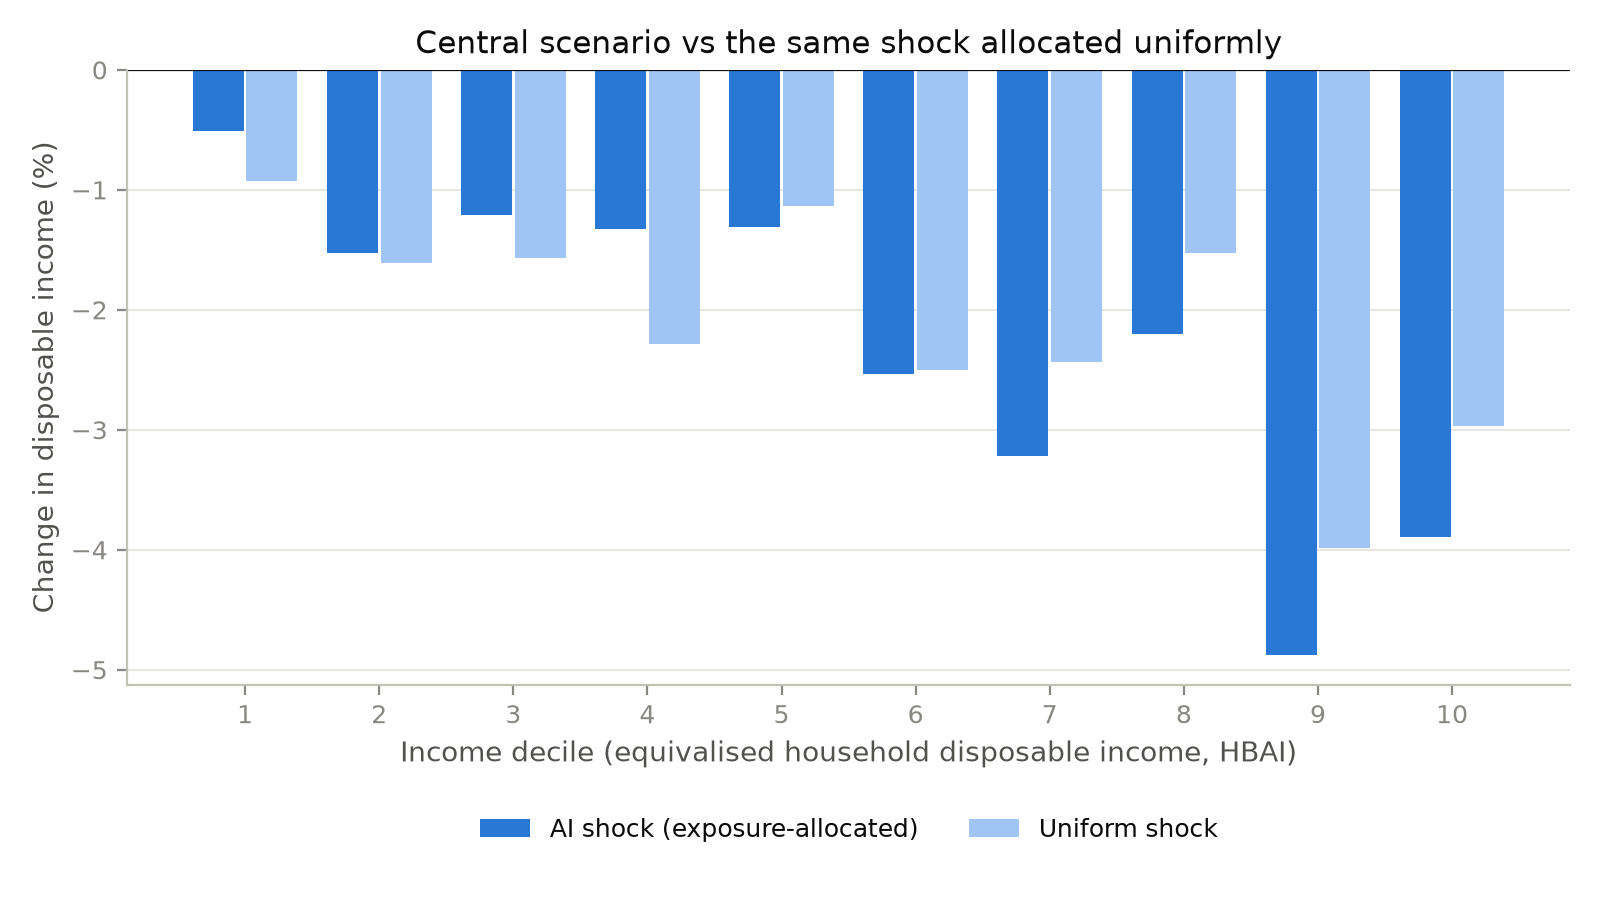
\includegraphics[width=.8\textwidth]{../results/appendix/b7_uniform_vs_ai_decile.png}
\caption{Disposable income change by decile: exposure-allocated versus uniform shock, central parameters.}
\label{fig:b7}
\end{figure}

\begin{figure}[htbp]
\centering
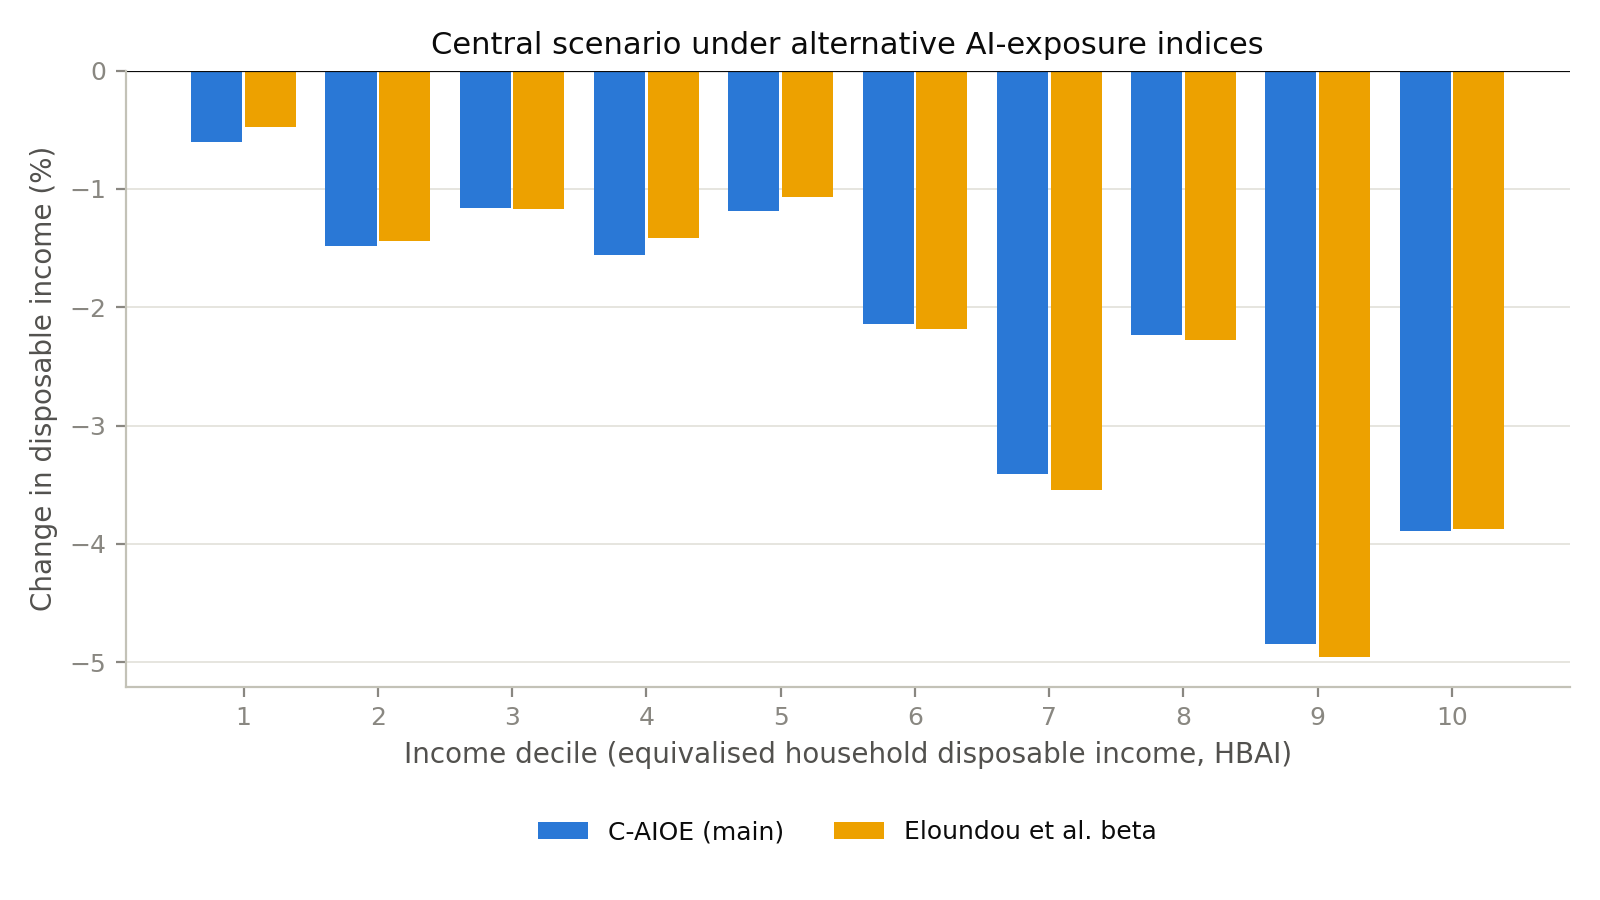
\includegraphics[width=.8\textwidth]{../results/appendix/b8_alternative_index_decile.png}
\caption{Disposable income change by decile under the C-AIOE and the Eloundou et al.\ exposure index.}
\label{fig:b8}
\end{figure}

\subsection{The scenario grid by decile, and without the capital shock}

Figure~\ref{fig:b9} facets the full 66-cell scenario grid by baseline
income decile; cells report the change in mean household disposable income
(HBAI concept), which across the grid as a whole ranges from $+3.0$ to
$-5.2$ per cent. Every decile's panel shifts towards losses as displacement
rises, but the top deciles darken much faster: in the harshest cell (10 per
cent displacement, no wage gain) the bottom decile loses 1.9 per cent of
disposable income while the top decile loses 8.2 per cent.
Figure~\ref{fig:b11} removes the capital-return shock. Average disposable
incomes fall relative to the capital-on grid, confirming that the capital
channel raises average incomes while concentrating its gains at the top;
the Gini result, however, is unchanged in kind: without the capital shock
the Gini of equivalised disposable income still rises in all 66 cells, by
0.00 to 1.50 percentage points. The inequality result does not depend on
the capital channel.

\begin{figure}[htbp]
\centering
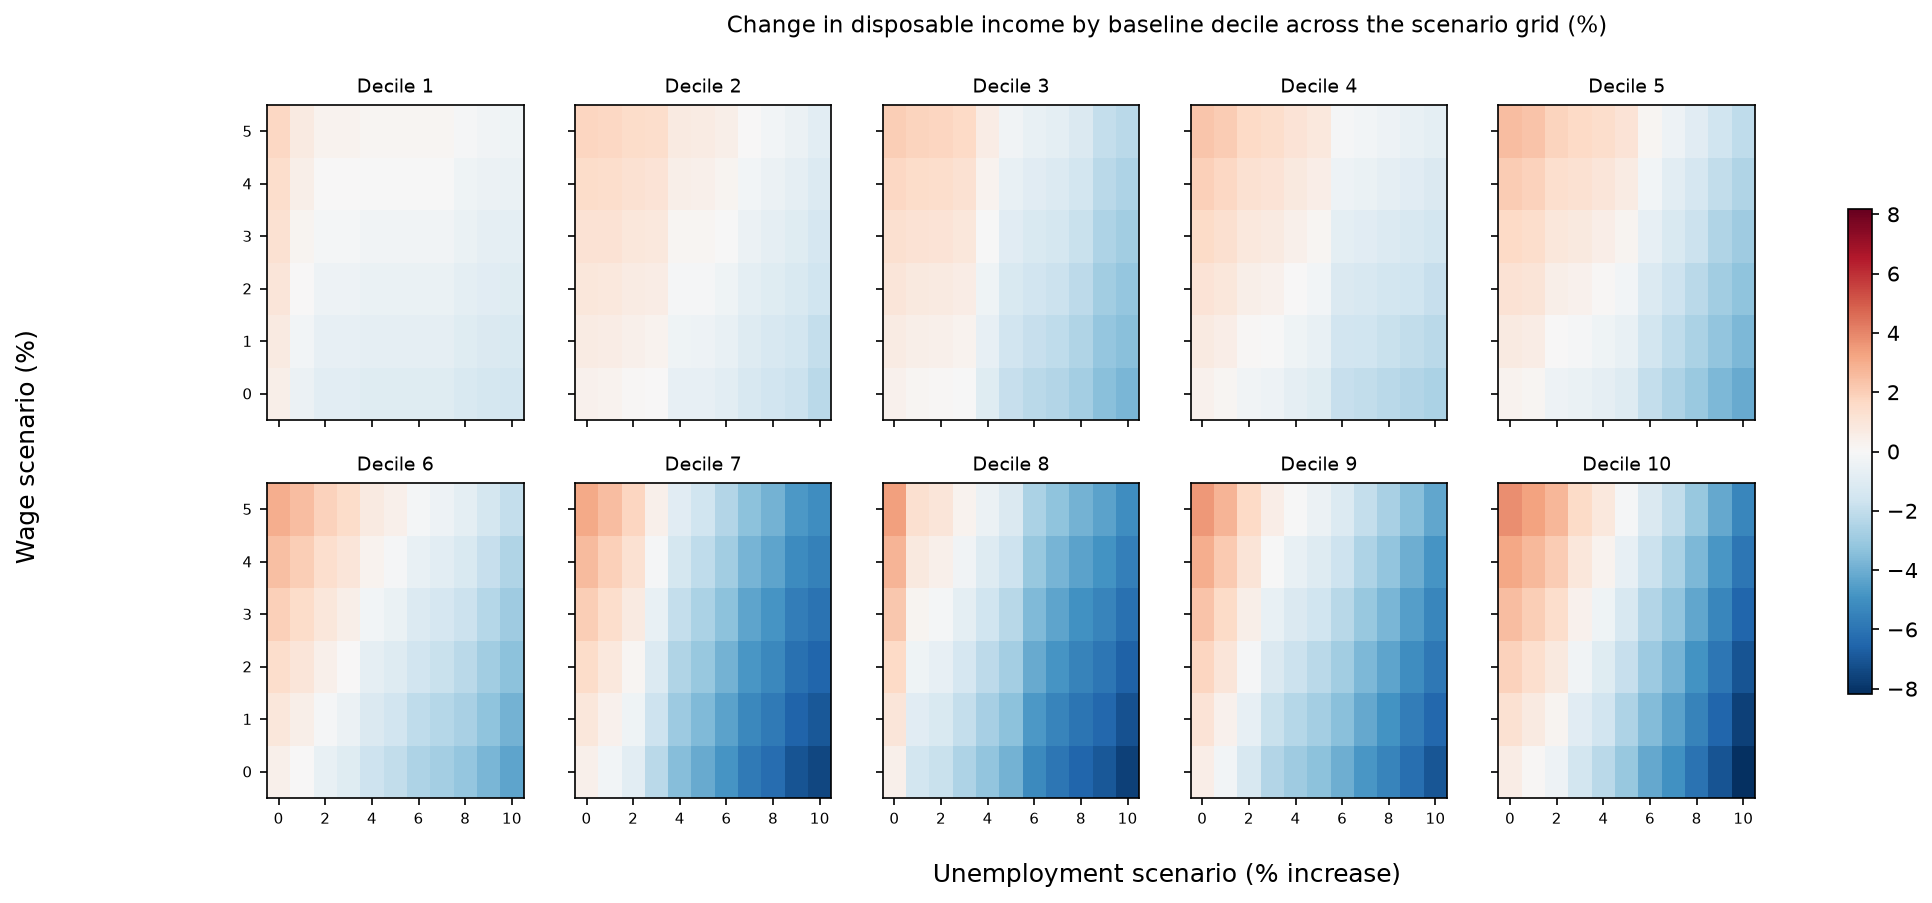
\includegraphics[width=\textwidth]{../results/appendix/b9_grid_by_decile.png}
\caption{Change in household disposable income across the scenario grid, faceted by baseline income decile. Single draw, seed 0.}
\label{fig:b9}
\end{figure}

\begin{figure}[htbp]
\centering
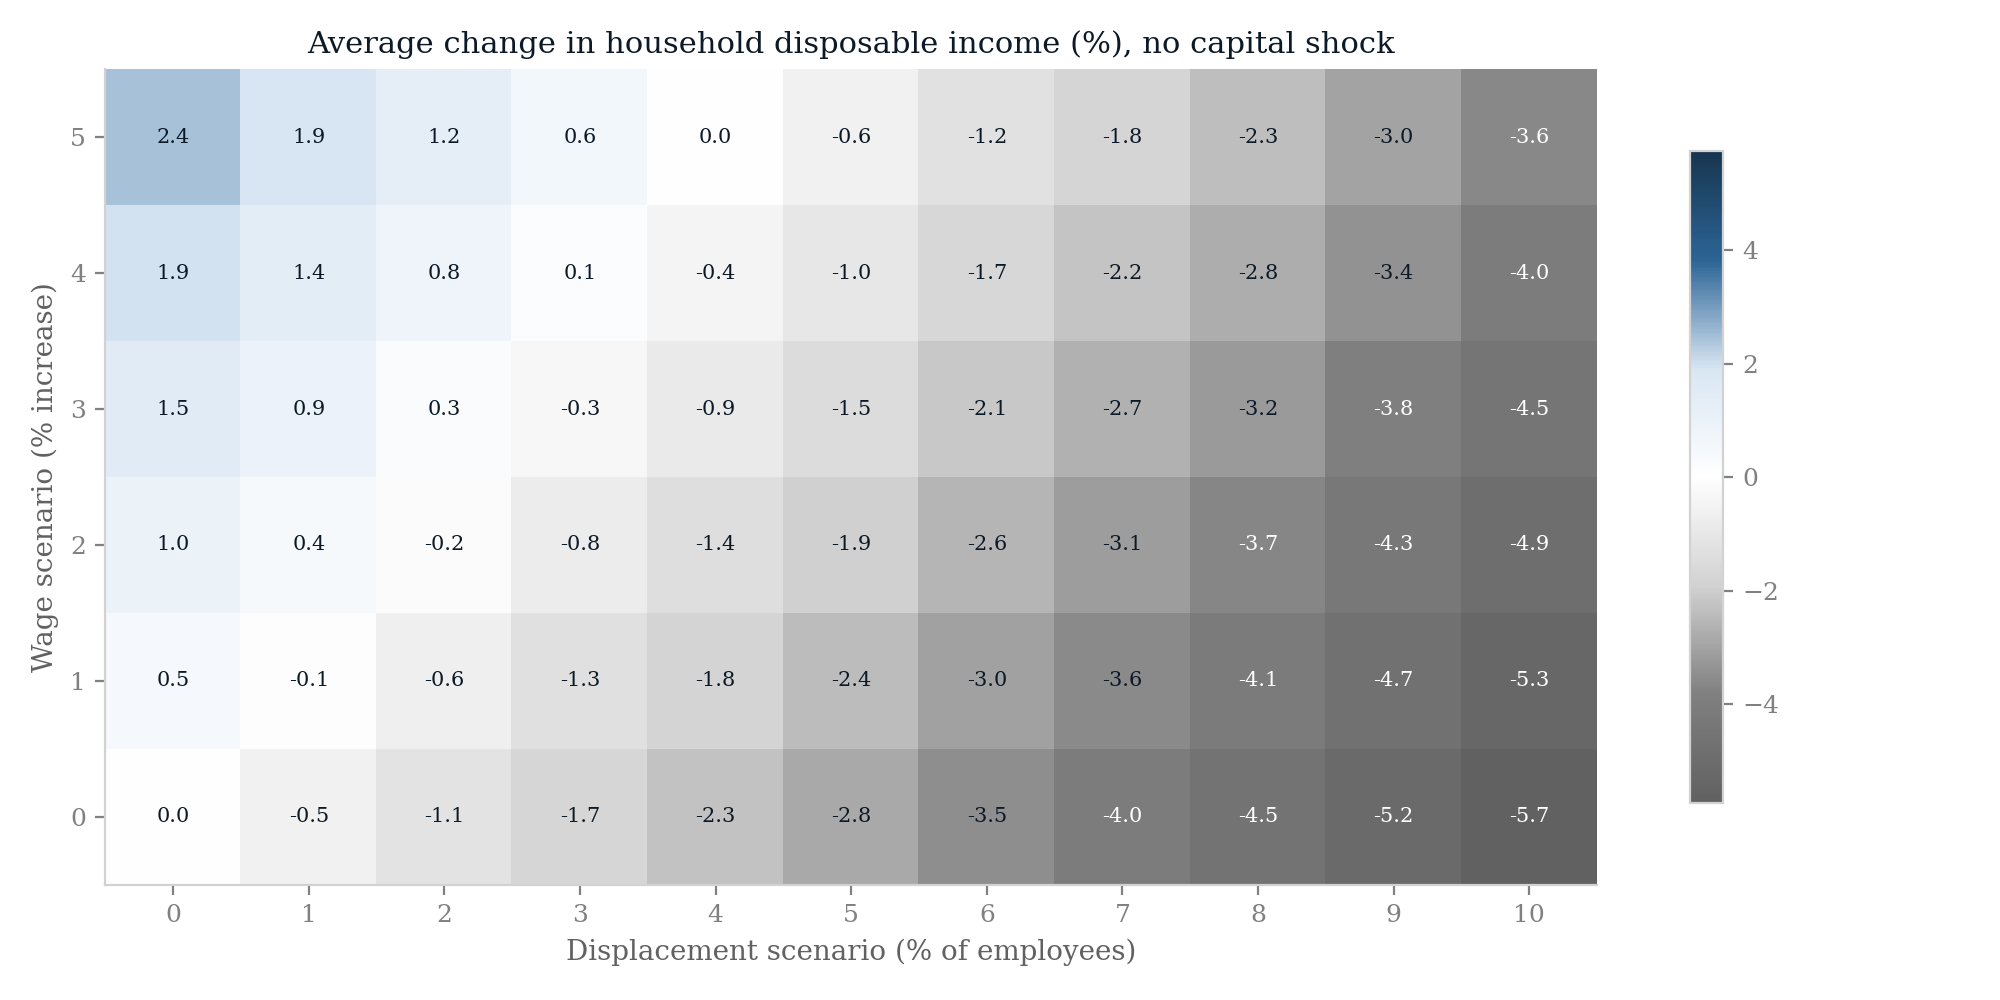
\includegraphics[width=.85\textwidth]{../results/appendix/b11_grid_no_capital.png}
\caption{Average change in household disposable income across the scenario grid with the capital-return shock switched off. Single draw, seed 0.}
\label{fig:b11}
\end{figure}


\end{document}
